\documentclass{article}

\usepackage{arxiv}

\usepackage[utf8]{inputenc} % allow utf-8 input
\usepackage[T1]{fontenc}    % use 8-bit T1 fonts
\usepackage[hidelinks]{hyperref}       % hyperlinks
\usepackage{url}            % simple URL typesetting
\usepackage{booktabs}       % professional-quality tables
\usepackage{amsmath,amssymb,amsthm}
\usepackage{amsfonts}       % blackboard math symbols
\usepackage{float}
\usepackage{nicefrac}       % compact symbols for 1/2, etc.
\usepackage{microtype}      % microtypography
\usepackage{mathrsfs}
\usepackage{onimage}
\usepackage{graphicx}
\usepackage{doi}
\usepackage{acronym}
\usepackage{listings}
\usepackage[mode=buildnew]{standalone}
\usepackage{tikz}
\usepackage{tabularx}
\usepackage{siunitx}
\usepackage{cite}
\usepackage{acronym}
\usepackage{xcolor}

\usetikzlibrary{calc}
\usetikzlibrary{shapes.geometric, arrows}

\tikzstyle{rect} = [
    rectangle,
    align=center,
    minimum width=3.1cm,
    minimum height=1cm,
    text centered,
    fill=color4!40,
    draw=color4dark,
    line width=1pt,
]
\tikzstyle{frect} = [rect, fill=color5!40, draw=color5dark]
\tikzstyle{brect} = [rect, fill=color1!40, draw=color1dark]
\tikzstyle{arrow} = [line width=1.2pt,->,>=stealth]
\tikzstyle{darrow} = [arrow, dashed]

\definecolor{color1}{HTML}{6bd2db}
\definecolor{color1dark}{HTML}{56a9b0}
\definecolor{color2}{HTML}{0ea7b5}
\definecolor{color3}{HTML}{0c457d}
\definecolor{color3dark}{HTML}{09325c}
\definecolor{color4}{HTML}{ffbe4f}
\definecolor{color4dark}{HTML}{cc993f}
\definecolor{color5}{HTML}{e8702a}
\definecolor{color5dark}{HTML}{ba5922}


\title{Methods for Analyzing Models of\\ Rod-Shaped Bacteria}

%\date{September 9, 1985}	% Here you can change the date presented in the paper title
%\date{} 					% Or removing it

\author{
    \href{https://orcid.org/0009-0001-0613-7978}{
        
\includegraphics[scale=0.06]{figures/orcid.pdf}
        \hspace{1mm}Jonas Pleyer
    }
    \thanks{
        \href{https://jonas.pleyer.org}{jonas.pleyer.org},
        \href{https://cellular-raza.com}{cellular-raza.com}
    }\\
	Freiburg Center for Data-Analysis and Modeling\\
	University of Freiburg\\
	\texttt{jonas.pleyer@fdm.uni-freiburg.de} \\
	%% examples of more authors
	\And
	\href{https://orcid.org/0000-0002-6371-4495}{
        
\includegraphics[scale=0.06]{figures/orcid.pdf}
        \hspace{1mm}Christian Fleck
    }\\
	Freiburg Center for Data-Analysis and Modeling\\
	University of Freiburg
}

\newacro{abm}[ABM]{Agent-Based Model}
\newacro{ode}[ODE]{Ordinary Differential Equation}
\newacro{pbr}[PBR]{Physically-Based Rendering}
\newacro{ib}[IB]{Individual-based}

% Define new units
\DeclareSIUnit\pixel{pix}

% Uncomment to remove the date
%\date{}

% Uncomment to override  the `A preprint' in the header
\renewcommand{\headeright}{Preprint}
%\renewcommand{\undertitle}{Technical Report}
\renewcommand{\shorttitle}{Methods for Analyzing Models of Rod-Shaped Bacteria}

\usepackage{enumitem}
\setlist{nolistsep}

%%% Add PDF metadata to help others organize their library
%%% Once the PDF is generated, you can check the metadata with
%%% $ pdfinfo template.pdf
\hypersetup{
pdftitle={% TODO
},
pdfsubject={q-bio.NC, q-bio.QM},
pdfauthor={Jonas Pleyer, Christian Fleck},
pdfkeywords={},
}

% Change numbering of equations
% \numberwithin{equation}{section}

% MAKE TITLES IN THEOREMS BOLD
\makeatletter
\def\th@plain{%
  \thm@notefont{}% same as heading font
  \itshape % body font
}
\def\th@definition{%
  \thm@notefont{}% same as heading font
  \normalfont % body font
}
\makeatother

\begin{document}
\maketitle


%###################################################################################################
\begin{abstract}
    \aclp{abm} have become popular tools in the study of complex cellular systems.
    However, despite their popularity, it is often difficult to systematically estimate their
    parameters and perform advanced analyses, e.g., using the profile-likelihood.
    In this work, we study the mechanical properties of rod-shaped bacteria and provide techniques
    for estimating their parameters and performing identifiability analysis on them.
    Our approach may serve as a blueprint for a modular framework which can be adapted to other
    research questions.
    We use time series of microscopic images as input data and incorporate advanced effects as the
    elasticity of the rod.
    The developed model serves as a generalized foundation to describe multiple species of
    rod-shaped bacteria such as \textit{E.Coli} or \textit{B.Subtilis}.
\end{abstract}

% keywords can be removed
% \keywords{}

\pagebreak
\renewcommand{\contentsname}{Table of Contents (remove before submission)}
\tableofcontents
\vfill
\pagebreak

%###################################################################################################
\section{Introduction}
\textbf{
    Mein Vorgehen: ich passe Formulierungen an, wenn ich im Prinzip mit der Aussage einverstanden
    bin, aber den Wortlaut verbesserungswürdig finde.
    Ich schreibe Kommentare, dort wo ich eher grundsätzliche Schwierigkeiten sehe.
    Dort wo ich nichts geändert habe und keinen Kommentar gegeben habe, kann ich zu einem späteren
    Zeitpunkt doch Änderungen vornehmen wollen.
}

\acp{abm} have proven to be powerfull tools in the study of complex cellular
systems~\cite{Pleyer2023}.
They have been applied in various scenarios, such as cancer
research~\cite{Ghaffarizadeh2018,Cooper2020}, Immuno-Oncology~\cite{Karolak2021} or the modeling
of mechanical intercellular connections in plant cells \textbf{TODO CITATION}.
By treating cells as individual entities, these tools allow researchers to think in terms of
cellular properties and processes thus allowing for a better understanding of the biological
reality.

Despite their popularity, \acp{abm} face multiple challenges in practise.
The construction of a fully functional \ac{abm} simulation from the ground up constitutes an
intricate and laborious process, necessitating a comprehensive array of skills. It is therefore
common practise to reuse existing simulation tools, which, in turn, brings along a number of
other problems.
Even if the existing tool is designed to be generalizable, it often comes with a pre-defined set
of parameters that need to be specified.
Furthermore, as we have discussed in our previous work~\cite{Pleyer2023}, these tools were most
often not designed to be flexible but rather built for specific purposes thus limiting their
generalizability \textbf{TODO CITATION}.
Typically researchers estimate the parameter of their model using methods such as Maximum Likelihood
or Maximum a Posteriori~\cite{Gbor2015,Banga2008,Ashyraliyev2009}, check for parameter
identifiability using methods like profile-likelihood or apply model reduction
techniques~\cite{Kreutz2013,Raue2014,Simpson2025}.

In the context of \acp{abm}, however, it is often only shown that the generated results lead to the
desired phenomenon aligning with the observed biological reality.
But this process does not actually estimate the necessary parameters directly \textbf{TODO CITATION}.
Consequently, it reduces the confidence in the constructed models and raises concerns with respect
to the validity of the obtained results.
In this work, we address these challenges using a general-purpose mechanical model for rod-shaped
bacteria as an example.
Our approach provides various methods which can be combined to systematically estimate the
parameters of our model. We deliberately distinguish between conceptually separate components within
this framework.
This modularity highlights a "blueprint" which can be adapted and applied to other \acp{abm}.

Mechanical properties of rod-shaped bacteria have been studied in great detail
experimentally~\cite{Chatterjee1988,Takeuchi2005,IWAI2002}.
It was found that the MreB protein is the driving force in maintaining their distinct elongated
shape~\cite{Ursell2014}, which plays an important role in the dynamics of
growth~\cite{Billaudeau2017}, division~\cite{Harry2001} and their collective
behaviour~\cite{vanGestel2015,Balagam2015}.
Furthermore, it has been discovered that the rod can be bent thus introducing temporary elastic or
permanent plastic deformations~\cite{Amir2014_2}.
Rod-shaped Bacteria are an interesting target system since their physical form provides more surface
information compared to other forms such as spherical cells.
In addition, parameters such as growth rates have been found to vary across multiple
cells~\cite{Koutsoumanis2013} which highlights the need to incorporate this heterogeneity on a
single-cell level.

Computational models for rod-shaped bacteria allow researchers to systematically analyze their
properties and infer emergent phenomena~\cite{Cho2007,Jnsson2005}.
Existing tools can describe growth, division and many effects such as colony formation and
expansion~\cite{Matyjaszkiewicz2017,Doumic2020} but they are limited in describing the
aforementioned plastic or elastic deformations of the rod. Furthermore, the literature on how to
estimate the parameters of such models directly from data is very sparse.

\textbf{
    Was mir hier nicht gefällt, ist, dass du von Parameter schätzen bei ABMs kommend ziemlich
    detailliert über Mechanik redest.
    Das passt nicht.
    Man erwartet mehr Infos über den Blueprint und ist verwirrt.
    Worum geht es hier?
}

This work addresses some of these limitations.
We use microscopic image time series as inputs to obtain information about the spatial configuration
of the cells.
This information can be used as initial values for a numerical simulation.
By varying the parameters of the model and comparing the results to the microscopic data, we can
estimate and quantify the parameters of our model.
Our approach takes a general stance which incorporates effects that are observed within
\textit{B.Subtilis} and \textit{E.Coli}.

%###################################################################################################
\section{Overview}
This work consists of many subcomponents which can be combined in order to achieve various tasks.
Figure~\ref{fig:flowchart-project-structure} shows a high-level overview of all components.
We assume that bacterial rods can be represented by a colleciton of vertices (see
section~\ref{subsec:spatial-representation}).
This assumption alone is enough to enable a cascade of other components.
Using the spatial representation, we provide visualization methods that create 3D models from the
given vertices which can then either be rendered or projected to a 2D plane.
The data extraction component determines the vertices from given cell masks which
correspond to microscopic images.
This allows us in particular to turn any sequence of images (movie) into a sequence of bacterial
positions.
The dynamics of the vertices are determined by a computational model which is specific
to the respective use-case and should be defined by the researcher.
It merely needs to utilize the aforementioned spatial representation of bacterial rods as a
collection of vertices.
This work will provide one example of how such a model can be defined.
Notably, the visualization and data extraction components do not require any knowledge about the
computational model, thus allowing us to reuse their functionality across multiple models.

Constructing a computational model requires knowledge about the target system and thus allows us to
interpret the results gathered by the provided data extraction methods.
These results can then further be used to restrict or determine the parameters of our model.
For example, by extracing the positions of bacteria across a time-series of microscopic images, we
can also calculate their lengths at these time-points and thus determine their rate of growth and
type of growth (see section~\ref{subsec:parameter-estimation-individual-treatment}), thus
effectively guiding our modeling steps.

Visualization methods are an integral part of any modeling endevaour.
They allow researchers to obtain feedback quickly and improve iteration times when constructing new
models. Furthermore, we utilize them in our more advanced parameter estimation methods (see
section~\ref{section:parameter-estimation}) where they enable us to effectively compare
two bacterial configurations across division events.
In the future, we are planning to build on the current state and generate realistic microscopic
images and time-series.
Together with the parameter estimation methods, they can then be used to provide large amounts of
mechanistic data for the training of cell-segmentation and cell-tracking machine-learning
algorithms.

\textbf{
    Du musst den Bogen hinbekommen von dem allgemeinen Problem des Parameterschätzen bei ABMs zu dem
    spezifischen Problem, welches du hier verhandelst.
}

\begin{figure}
    \centering
    % \includegraphics[width=0.8\textwidth]{overview.pdf}
    \includestandalone[width=0.8\textwidth]{figures/concept/overview}
    \caption{
        The project can be divided into subcomponents (yellow, red) that interact with and depend on
        each other.
        Yellow blocks are provided by this work and red blocks require additional input such as
        modeling assumptions or data.
        Blue blocks indicate possible future extensions of this project.
        Every component implicitly builds on the spatial representation of rod-shaped bacteria as
        vertices.
    }
    \label{fig:flowchart-project-structure}
\end{figure}

%###################################################################################################
\section{A Computational Model for Rod-Shaped Bacteria}
\label{sec:computational-model}

The mechanical behaviour of rod-shaped bacteria is governed by a plethora of effects.
In this work, we aim to establish a model which is general enough such that it can be reused as the
basis for many variants of rod-shaped bacteria but also explicit enough such that we can quantify
its parameters.
We thus utilize only a minimal set of assumptions.

When describing the bacterial system, we distinguish between intra-cellular processes and cell-cell
interactions.
We restrict ourselves to the features discussed below and summarize them in
Table~\ref{table:simulation-aspects}.
% For a collection of other known aspects which could be considered, we refer to the supplementary
% section~\ref{section:discussion}, and~\ref{section:supplement-more-simulation-aspects}.

While some rod-shaped bacteria grow by inserting new material at the ends, \textit{E.Coli} and
\textit{B.Subtilis} utilize a method where new material is inserted along the cylindrical part of
the rod. The details of the division event (i.e. Z-Ring formation) are very intricate and are heavily
studied as a subject on their own~\cite{Harry2001}.
On a higher level view, the rod is split apart at a point close to the center of the cell, thus
creating two new daughter cells.
It was shown that the best predictor for when the division event occurs, is the length of the rod as
opposed to the age of bacterium~\cite{Robert2014}.
Furthermore, not only the growth of the whole colony but also the growth of individual bacteria is
exponential~\cite{Amir2014,Takeuchi2005}.
The growth rates of individual bacteria and other process parameters can be heterogeneous which
should be accounted for as well \cite{Koutsoumanis2013}.

Many bacteria organize into biofilms~\cite{Dunne2002,Ong1999} which play a key role in the survival
of the collective.
Their formation is only possible due to the attractive nature of bacterial interactions between
each other~\cite{Berne2018}.
This interaction is characterized by a long-range attraction and short-ranged
adherance~\cite{Verwey1947,Trejo2013}.
We therefore need account for this phenomenon as well.

\begin{table}[H]
    \centering
    \def\arraystretch{1.3}
    \begin{tabularx}{\textwidth}{c l X}
        &\textbf{Aspect} & \textbf{Description}\\
        \toprule
        &\textbf{(C) Cellular}\\
        \midrule
        (1) & Rod-Shaped Mechanics &
            Rod-shaped bacteria are flexible rods which are able to freely move around (off-lattice
            approach) \cite{Takeuchi2005,Ursell2014,Amir2014_2}.\\
        (2) & Growth &
            Cells grow exponentially by inserting new material either along the circular part of the
            rod or at the tip~\cite{Robert2014,Takeuchi2005}.\\
        (3) & Division &
            Rod-Shaped bacteria divide in the middle of the rod into two new agents.\\
            % Bacteria can form multilayers during their growth phase \cite{Duvernoy2018}.\\
        &\textbf{(CC) Cell-Cell Interactions}\\
        \midrule
        (4) & Adhesion &
            Bacteria attract at longer distances and adhere to each other at shorter
            distances~\cite{Verwey1947,Trejo2013}.\\
        \bottomrule
    \end{tabularx}
    \caption{
        This table lists aspects of cellular behaviour which we consider in our computational model.
        It is split into cellular aspects (C) which concern only an individual bacterium and
        interactions between cells (CC).
        These aspects are generalized in order to fit to as many types of rod-shaped bacteria as
        possible.
        These are the assumptions for the basic model that we are presenting here.
        In order for our methods to work, we are really only required to satisfy the assumption of
        our spatial representation (see section~\ref{subsec:spatial-representation}) and thus, these
        assumptions can also be loosened if required.
    }
    \label{table:simulation-aspects}
\end{table}

% --------------------------------------------------------------------------------------------------
\subsection{Spatial Representation}
\label{subsec:spatial-representation}
This work makes use of a few but powerful assumptions concerning the mathematical representation of
the cells. In order to describe the spatial dynamics of individual cells or agents, we need to
define their position, shape and how they interact with each other.

In order to provide as much flexibility as possible when constructing new models, we restrict
ourselves to assumptions concerning the position such that researchers can freely experiment with
various shapes and interaction types.
\textbf{[Dieser Satz ist leider unverständlich. Je öfter ich den Satz lese, umso weniger ist mir klar, was du sagen möchtest.]}\\


Furthermore, it is very important to strike a good balance between the restrictiveness of our
assumptions and generality in order to provide meaningful results and still be able to apply our
approach to a broader class of models.
\textbf{[Ebenso unklar warum du das hier an dieser Stelle sagst. Vielleicht versuchst du die Aussagen zu bündeln und geeigneter Stelle zu bringen. So ist man leider eher verwirrt.]}\\

Taking into account the natural shape of rod-like bacteria, it is clear that they can not be
represented with a singular point $\vec{x}$ in space.
\textbf{[Hast du nicht bereits oben die Hilfsvariablen $x_i$ eingeführt?]}\\

We could extend this positional definition with a vector $\vec{w}$, indicating the direction of
extension but this would restrict ourselves to fully straight rod-shaped bacteria.
\textbf{[Nicht spekulieren was du hättest machen können, sondern einfach sagen, was du gemacht hast.]}

However, multiple experiments have shown that MReB is responsible for the growth and maintenance of
the elongated shape of bacteria~\cite{Erickson2001}.
\textbf{[Wiederholung?]}


By means of this protein, rod-shaped bacteria can bend elastically on short time-scales and deform
plastically over longer periods of time. Our goal is to provide a model that can encapsulate these effects.
\textbf{[Das beschriebene Verhalten ist visko-elastisch. Soweit ich sehe, hast du das nicht implementiert. Könnte es sein, dass das elastisches Modell mit Wachstum äquivalent zum Maxwell-Modell ist? Eigene Antwort: im allgemeinen nein.]}\\

We discretize the (possibly non-straight) rod of a bacteria and model it by using multiple vertices
which are part of a 1-dimensional
polygon with two endpoints $\vec{x}_i$. \textbf{[Was ist denn die Diskretisierungslänge? Two endpoints $x_i$ macht keinen Sinn.]}\\

Figure~\ref{fig:mechanics-bacterium} shows a visualization of this approach.
The angles $\alpha_i$ between vertices $\vec{x}_{i-1},\vec{x}_i$ can be used when modeling the
dynamics of these bacteria.
\textbf{[Klingt kryptisch. "Can be used ..". Für was, wie?]}\\

With these fundamental thoughts layed out, we retain the flexibility to represent many models such
as varying shapes since we do not have to make any assumptions on the type of interactions between
two bacteria.
Even concerning the shape of bacteria, this assumption still allows us to model elliptical cells by
modifying the interaction type as well as other effects such as polarity of
interactions~\cite{Duvernoy2018}.
Furthermore, we also did not have to assume any particular mechanical dynamics of the agents, only
their spatial representation, thus leaving in particular room for plastical or elastic deformations
of the rod and other more intricate mechanisms.
\textbf{[Ich glaube, ich verstehe warum du das hier sagst. Aber das kommt nicht richtig rüber. Der Absatz ist vielleicht nicht nötig. Der Kommentar über elliptische Zellen, sollte eher unter Potential stehen?]}\\

% \begin{enumerate}
%     \item represent bacteria as polygon with vertices $\vec{x}_i$
%     \item Assumes that these vertices are not fundamental but rather a discretization of the actual
%         problem
% \end{enumerate}

\begin{figure}
    \centering
    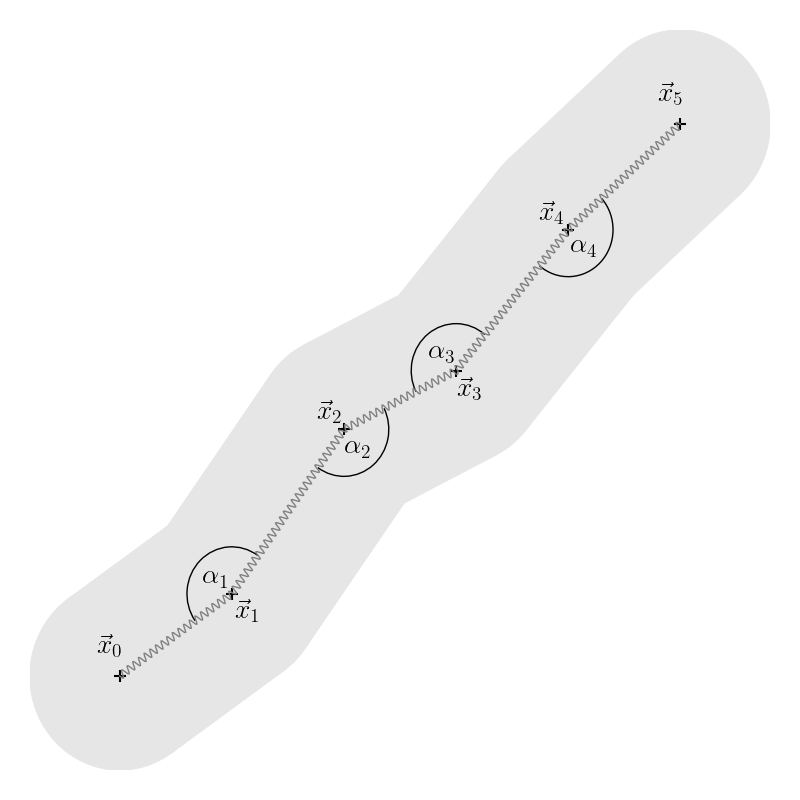
\includegraphics[width=0.5\textwidth]{docs/source/_static/mechanics.png}
    \caption{
        Example of an elonged bacterial rod represented by a collection of vertices which are
        connected by springs.
        The angles $\alpha_i$ have been exaggerated such that they can be identified more easily.
        A bacterial agent which is not interacting with any external objects will tend to the
        equilibrium state of a straight rod with no curvature.
    }
    \label{fig:mechanics-bacterium}
\end{figure}

% --------------------------------------------------------------------------------------------------
\subsection{Mechanics}
\label{subsection:mechanical-model-mechanics}
We use principles from discrete differential geometry~\cite{bobenko2008discrete} to describe the
stiffness of the bacterial rod~\cite{Amir2014_2}.
As explained above, MReB will counteract the bending of the rod, resulting in a stiffening force.
In principle, this stress will be dependent on the position inside the cell~\cite{Chatterjee1988},
but for sake of simplicity we chose to model the bacterium as a bending beam.
\textbf{[", thus utilizing the simplest solution which can still produce the desired effects." Es ist unklar was die "desired effects" sind. ]}\\

Such a beam can be represented by a collection of vertices $\vec{x}_i$ which are connected by a
springs of lengths $l_i$.
\textbf{[Das klingt nach einer Wiederholung von Spatial Representation. Du erklärst ziemlich umständlich. Konzentriere dich auf das wesentliche und überlege, was du eigentlich sagen möchtest.]}\\

We use the notation $\vec{c}_i:=\vec{x}_i-\vec{x}_{i-1}$ with which the resulting force acting
between two vertices if given by

\begin{align}
    \vec{F}_{i,\text{springs}} =
        &-\gamma\left(1 - \frac{l}{\left|\vec{c}_i\right|}\right)
        \vec{c}_i\\
        &+ \gamma\left(1 - \frac{l}{\left|\vec{c}_{i+1}\right|}\right)
        \vec{c}_{i+1}.
\end{align}

The value of the spring constants determines the elasticity with respect to elongation of the cell.
In situations where this aspect is not relevant, they merely serve as a auxiliary parameters to
maintain the length of the rod.
In addition to springs between individual vertices $\vec{x}_i$, we assume that each angle at a
vertex between edges is subject to a force indiced by curvature.
% We assume that we can model the mechanical properties of the bacterium as an elastic rod.
Given the angle $\alpha_i = \sphericalangle(\vec{c}_{i-1},\vec{c}_i)$ between adjacent edges,
the bending force is proportional to the curvature $\kappa_i$ at each vertex
$\kappa_i = 2\tan(\alpha_i/2)$.
The resulting force acts along the angle bisector which can be calculated from the edge vectors.
Figure~\ref{fig:mechanics-bacterium} shows an elongated rod represented by $6$ vertices.
The forces acting on vertices $\vec{x}_i,\vec{x}_{i-1},\vec{x}_{i+1}$ are given by

\begin{align}
    \vec{F}_{i,\text{curvature}} &= \eta\kappa_i
        \frac{\vec{c}_i - \vec{c}_{i+1}}{|\vec{c}_i-\vec{c}_{i+1}|}\\
    \vec{F}_{i-1,\text{curvature}} &= -\frac{1}{2}\vec{F}_{i,\text{curvature}}\\
    \vec{F}_{i+1,\text{curvature}} &= -\frac{1}{2}\vec{F}_{i,\text{curvature}}
\end{align}

where $\eta_i$ is the rigidity at vertex $\vec{x}_i$ (see Figure~\ref{fig:mechanics-bacterium}).
We can see that the curvature force does not move the overall center of the rod in space.
The total force is the sum of external and interal forces.

\begin{equation}
    \vec{F}_{i,\text{total}} = \vec{F}_{i,\text{springs}}+ \vec{F}_{i,\text{curvature}}
        + \vec{F}_{i,\text{external}}
\end{equation}

and are integrated via damped brownian dynamics

\begin{align}
    \partial_t^2 \vec{x}_i &= \partial_t\vec{x}_i + \sqrt{2D}\vec{\xi}_i\\
    \partial_t\vec{x}_i &= \vec{F}_{i,\text{total}} - \lambda \partial_t\vec{x}_i
\end{align}
\textbf{[Ich verstehe die Gleichungen nicht. Eine überdämpfte Langevin Gleichung bezeichnet man doch als Brownsche Bewegung, oder? Und sollte die Brownsche Gleichung nicht so lauten?
\begin{align}
   \partial_t \vec{x}_i &= \frac{D}{k_B T} \vec{F}_{i,\text{total}} + \sqrt{2D}\vec{\xi}_i
\end{align}
Die Einheiten stimmen auch überhaupt nicht. $[x_i]=$m, $[\lambda]=$kg/s, $[F]=$(kg m)/s$^2$
]}\\

where $D$ is the diffusion constant, $\vec{\xi}$ is a Wiener process and $\lambda$ a damping constant.
Together they determine the stochastic motion of the individual vertices which can arise from
recurring collisions with small particles of the surrounding medium or other minor fluctuations.

% --------------------------------------------------------------------------------------------------
\subsection{Physical Interactions - Mie Potential}

Calculating the force between cells resulting  from long ranged interactions requires performing a
double integral over the length of the cells. 
To reduce the computational costs we use a approximative, simplified model Given a vertex
$\vec{x}_i$ on one cell, we determine the closest point $\vec{p}$ on the polygonal line given by the
vertices $\{\vec{w}_j\}$ of the interacting cell. 
\textbf{[Ich bin etwas verwirrt. Warum änderst du die Bezeichnung der Vertices?]}

Furthermore we determine the value $q\in[0,1]$ such that $\vec{p} = (1-q)\vec{w}_j + q\vec{w}_{j+1}$
for some specific $j$.
The force is then calculated between the points $\vec{x}_i$ and $\vec{p}_i$ and acts on
the vertex $\vec{w}_i,\vec{w}_{i+1}$ with relative strength $(1-q)$ and $q$.

\begin{equation}
    \vec{F}_{i,\text{External}} = \vec{F}(\vec{x}_i,\vec{p})
\end{equation}

The interaction between cells can be described by the Mie potential~\cite{Mie1903}.
It is the generalization of the well-known Lennard-Jones~\cite{Jones1924} potential and was designed
to describe the interactions between molecules.
The Mie potential is given by:

\begin{align}
    U(r) &= C\epsilon\left[ \left(\frac{\sigma}{r}\right)^n -
        \left(\frac{\sigma}{r}\right)^m\right]\\
    C &= \frac{n}{n-m}\left(\frac{n}{m}\right)^{\frac{n}{n-m}}\\
    V(r) &= \min(U(r), \beta)\theta(r-\zeta)
\end{align}

The strength of the potential is given by $\epsilon$ and the radius \textbf{[Welcher Radius?]} is
encoded in $\sigma = (m/n)^{1/(n-m)}(R_1+R_2)$ where $R_1,R_2$ are the radii of the two interacting
particles.
In our simulation, we use $V(r)$ to guarantee numerical regularity.
\textbf{[Beschreibe, welche Rolle $\beta$ und $\zeta$ spielen.]}

The specific choice of interaction potential plays a crucial role for the dynamics of the agents.
Since we cannot expect to simply know the correct shape and parameters of this potential, it is
desirable to experiment with various interaction potentials in order to quantify their
ability to produce accurate results.
While this study, only relies on the Mie Potential, our python package \texttt{cr\_mech\_coli}
also implements the popular Morse potential~\cite{Morse1929} to model physical interactions.

\textbf{[Du hast hier von shape geredet. Das Potential ist doch immer radial-symmetrisch, oder? Vielleicht könnte es helfen, Bilder zu zeigen? Darin könnte man die Bedeutung der Parameter verdeutlichen. Wenn du schreibst, das Potential ist sehr wichtig, dann musst du viel besser begründen, warum du das Potential gewählt hast. Ich denke, du solltest das etwas abschwächen.]}

% --------------------------------------------------------------------------------------------------
\subsection{Cell-Cycle}

To simulate proliferation, we introduce a growth term for the spring lengths $l_i$.
In most of our simulations, we choose to use identical lengths for all segments (i.e. $l_i=l$).
However, in order to generalize our approach we assume that individual lengths of segments could
vary. Our implemented model allows us to reduce the growth rate with increasing number of neighbours
$n\leq N$. This option provides a phenomenological approach for modelling slower growth in larger colonies but
is be toggled off by default thus removing the additional term in brackets of equation~\ref{eq:growth-rod-lengths}.

\textbf{[Ich empfinde deinen Text als uneinheitlich. Du solltest hier nicht deine Softwareimplementation beschreiben, sondern das was du tatsächlich in den Simulationen benutzt hast. Also Möglichkeiten, die du in deinem Code angelegt hast, aber für das Paper nicht verwendet hast, brauchst du nicht zu erwähnen. Das führt zu Verwirrung.]}

\begin{equation}
    \partial_t l_i = \mu\left(1-\frac{\text{min}(n,N)}{N}\right)l_i
    \label{eq:growth-rod-lengths}
\end{equation}

Note that the growth rate is proportional to the rod length $l$ which leads to exponential
growth~\cite{Robert2014,Takeuchi2005}.
\textbf{[Das zu erwähnen ist eine Trivialität für ein Forschungspapier. Du kannst begründen warum du exp. Wachstum verwendest und wie du den Teilungszeitpunkt bestimmst.]}

This process will increase the length of the cell indefinitely unless we impose a condition for the
division event. We define a fixed length threshold for the total length of the cell at which it divides.
To construct a new cell, we cannot simply copy the existing one twice, but we also need to adjust
internal parameters in the process.
The following actions need to be taken for the old and new agent.
We first calculate the new spring lengths of the two resulting rods, according to the equation:

\begin{equation}
    \tilde{l} = l_i\left(\frac{1}{2} - \frac{r}{\sum\limits_i l_i}\right)
    \label{eq:growth-rod-new-lengths}
\end{equation}

Afterwards, we start at one endpoint $\vec{x}_0$ and move along the polygon defined by the
bacterial rod. We stop when we have reached a length that matches the length of the new spring length $\tilde{l}$.
From here, we continue and iterate this procedure until we have found all new vertices $\vec{w}_i$.
Equation~\ref{eq:growth-rod-new-lengths} ensures that that the tips of the two new rods are touching
right after the division event.
\textbf{[Was ist $r$? Was ist mit den Parametern und mit anderen intro-zellularen Zuständen?]}

% --------------------------------------------------------------------------------------------------
\subsection{Numerical Implementation}

We implemented the described model in our recently developed \ac{abm} framework
\texttt{cellular\_raza}~\cite{Pleyer2025}.
By design \texttt{cellular\_raza} does not assume any particular cellular representation, thus makes
it flexible and easy to adapt the simulation to particular needs. This allows us to experiment with
different model implementations and still retain performance.
\textbf{[Der Zusammenhang zwischen der Flexibilität und Performance ist unklar.]}

Furthermore, it is an \ac{abm} which is able to natively track cells through the course of a
numerical simulation and also keeps track of mother/daughter relationships.
\textbf{[Das scheint hier trivial zu sein.]}

On the programming side, we are using the \texttt{pyo3} and \texttt{maturin} crates which allow us
to easily generate Python bindings and enable us to interoperate between the two ecosystems.
\textbf{[Das kennt hier keiner und gehört eher in den Anhang.]}

By using \texttt{cellular\_raza}, we can make use of multiple threads for running a single numerical
simulation, using the built-in parallelization methods (see Supplementary Material,
Figure~\ref{fig:performance}).
\textbf{[Ist alles eher für den Anhang. Vielleicht solltest du mehr darüber reden, warum ABMs für die Fragestellungen gut geeignet sind.]}

%###################################################################################################
\section{Methodology}
These sections introduce methods which can be combined in order to estimate the parameters of our
computational model.
It has to be noted that they only depend on the spatial representation described in
section~\ref{subsec:spatial-representation}.
Consequently, these models can be applied to a broader class of mechanical models that may exhibit
varied cellular behaviours.

% --------------------------------------------------------------------------------------------------
\subsection{Visualization}
\label{subsection:visualization}
To visualize the spatial configuration of the results we employ pyvista, which provides high-level
wrappers around the popular VTK library~\cite{vtkBook,Sullivan2019}.
The initial phase of the visualization process entails the generation of three-dimensional meshes
for each bacterium as an intermediate representation.
We insert spheres of a given radius $r$ at each vertex $\vec{x}_i$ and connect adjacent vertices
$\vec{x}_i,\vec{x}_{i+1}$ with a cylinder, also of radius $r$ which is positioned such that its core
is identical to the connecting line segment between the two vertices.
Finally, we combine the meshes of all of these objects to obtain a single mesh of one bacterium.

A render of this result can be seen in figure~\ref{fig:progression-image-generation}.
Since we use a 3D rendering engine as an intermediate representation, the resulting image can have
overlaps of bacteria which are placed at higher or lower values along the z-direction.
To generate masks, we assign unique colours to every mesh of the respective cellular agent, ensuring
no two agents will use identical colours.
We then use a parallel projection and remove any existing light sources in order to obtain a solid
color for every cell-agent.
The resulting image is shown in subfigure (B).
Subfigure (C) shows an example of a simplified way to generate microscopic images.
The properties of the meshes such as roughness and reflectivity have been adjusted and we use
physically-based rendering of VTK. The result of this render is augmented by introducing white noise
on the pixel values at each point.
\textbf{[Warum?]}

This approach is very rudimentary and we hope to extend these methods in the future.
\textbf{[So sollte man das nicht formulieren. Hört sich etwa so an wie: jetzt hatte ich keine Lust es richtig zu machen, aber vielleicht mache ich das in der Zukunft.]}
In order to properly generate data, we need to deal with microscopic imaging techniques and possible
defects that can occur. It is crucial to get this part of the image-generation process right in
order to obtain near-realistic images that can be further reused.
\textbf{[Kann wenig mit diesen Kommentaren anfangen. Verstehe nicht warum du das hier sagst.]}

% \begin{itemize}
%     \item use pyvista (VTK) for Visualization
%     \item always do 3D render. This way, we can have overalp between agents and produce more
%         realistic masks.
%     \item Assign unique color values for idividual agents.
%         We have a 1:1 mapping between agent identifier and color! (for each simulation different
%         though)
%     \item use parallel projection; this should be most close to what microscopes measure due to the
%         relatively large distance between object and lens.
%     \item use some noise to smear out the rods; this is already similar to microscopic images; use
%         more like this and deal with real-world defects to make it more realistic (future, not now)
%     \item Figure~\ref{fig:progression-image-generation} shows steps in generating image.
%     \item Reflectivity, placement of light etc. can already introduce some heterogeneity in the
%         visual of the rod.
%     \item Plan to implement noise on the mesh itself; make it have rough surface (like real rods as
%         seen under electron microscopy)
% \end{itemize}
%
% \paragraph{Algorithm}
% \begin{enumerate}
%     \item Get position of cell
%     \item Insert spheres at each vertex
%     \item Insert cylinder along edges
%     \item Combine individual objects into one big mesh
%     \item Use \ac{pbr}
% \end{enumerate}

\begin{figure}
    \centering
    % \begin{tikzonimage}[width=0.9\textwidth]{visualization.pdf}
    %     \node at (0.025, 0.975)[anchor=north west, rectangle, draw, minimum width=15pt, minimum height=15pt]{\textbf{A}};
    % \end{tikzonimage}
    \begin{tikzonimage}[width=0.3\textwidth]
        {docs/source/_static/09395645494836445480/raw_pv/000000400.png}
        \node at (0.025, 0.975)[anchor=north west, rectangle, draw, white, minimum width=15pt, minimum height=15pt]{\textbf{A}};
    \end{tikzonimage}
    \begin{tikzonimage}[width=0.3\textwidth]
        {docs/source/_static/09395645494836445480/masks/000000400.png}
        \node at (0.025, 0.975)[anchor=north west, rectangle, draw, white, minimum width=15pt, minimum height=15pt]{\textbf{B}};
    \end{tikzonimage}
    \begin{tikzonimage}[width=0.3\textwidth]
        {docs/source/_static/09395645494836445480/images/000000400.png}
        \node at (0.025, 0.975)[anchor=north west, rectangle, draw, white, minimum width=15pt, minimum height=15pt]{\textbf{C}};
    \end{tikzonimage}
    \caption{
        (A) shows the result from combining sphere and cylinder meshes to obtain the shape of a
        bacterial rod.
        This render contains lighting coming from 2 light sources which thus produces a small glow
        on the upper part of the meshes.
        (B) Unique color values are assigned to each agent and light sources are removed.
        Afterwards, the image is rendered by projecting along the z-axis.
        (C) We use physically-based rendering and assign properties such as roughness and
        reflectivity to generate an initial render.
        Afterwards, we apply white noise to the pixel values of image.
        In the future, we hope to extend this approach in order to construct near-realistic
        microscopic images from synthetic data.
    }
    \label{fig:progression-image-generation}
\end{figure}

% --------------------------------------------------------------------------------------------------
\subsection{Data Extraction}
\label{section:data-extraction}

This section will explain how we can determine the collection of vertices $\vec{x}_i$ introduced in
subsection~\ref{subsection:mechanical-model-mechanics} from microscopic images
(Figure~\ref{fig:position-extraction-algorithm} (A)).
They will serve as initial, final and intermediate values with which we can compare our predictions.
\textbf{[Beziehen sich initial und final, usw. auf räumliches? Ist missverständlich, bitte umformulieren.]}
The algorithms which we devised requires the input of cell-masks which assign a unique color for
every cell in the image.

Such masks can be generated by cell-segmentation tools or obtained by annottating microscopic images
by hand (Figure~\ref{fig:position-extraction-algorithm} (B)).
Afterwards, we proceed with the following 5 steps.
\begin{enumerate}
    \item Obtain submasks for each cell individually.
    \item Skeletonize submask with algorithm from Lee~\cite{Lee1994}
    \item Determine endpoints $\vec{q}_0,\vec{q}_1$.
        Assert that there are only 2 endpoints.
        \textbf{[Heissen die Endpoints immer $q$? Kontrolliere bitte, ob deine Notation einheitlich ist.]}
    \item Sort points such that they form a polygon.
    \item Interpolate vertices $\vec{x}_i$ from obtained polygon.
\end{enumerate}

In the first step, the image will be split into a collection of subimages that only contain
information for one single cell.
From there, we apply a skeletonization algorithm~\cite{Lee1994}
(Figure~\ref{fig:position-extraction-algorithm} (C)).
It has to be noted that there are multiple variants of skeletonization and in general, these classes
of algorithms can produce results which have intersection points and multiple endpoints, which is
undesirable in our case.
We have found that for most practical examples, the algorithm devised by~\cite{Lee1994} works well.\\

The skeletonization algorithm supplies us with a collection of unordered lattice points $\vec{p}_i$
(pixel coordinates) where the skeleton lives.
We identify the endpoints $\vec{q}_0,\vec{q}_1$ by counting the number of neighbors in the von
Neumann neighborhood for each lattice point.
Any point with exactly one neighboring point must be and endpoint.
If we encounter more or less than two points which fit this criterion, the routine can not commence
and is aborted.
Next, we start with one of the endpoints and determine the next neighbor which was not yet picked.
We list the points in this order, thus forming a sorted polygon of pixel coordinates.\\
In the last step, we take the sorted, extracted points $\vec{p}_i$ and interpolate $n$ values for
the desired number of vertices $\vec{x}_i$.

\begin{figure}
    \centering
    \begin{tikzonimage}[width=0.36\textwidth]
        {docs/source/_static/fitting-methods/algorithm/image001042.png}
        \node at (0.025, 0.975)[anchor=north west, rectangle, draw, white, minimum width=15pt, minimum height=15pt]{\textbf{A}};
    \end{tikzonimage}
    \begin{tikzonimage}[width=0.36\textwidth]
        {docs/source/_static/fitting-methods/algorithm/mask-zoom.png}
        \node at (0.025, 0.975)[anchor=north west, rectangle, draw, white, minimum width=15pt, minimum height=15pt]{\textbf{B}};
    \end{tikzonimage}
    \begin{tikzonimage}[width=0.255\textwidth]
        {docs/source/_static/fitting-methods/algorithm/interpolate-positions.png}
        \node at (0.025, 0.975)[anchor=north west, rectangle, draw, white, minimum width=15pt, minimum height=15pt]{\textbf{C}};
    \end{tikzonimage}
    \caption{
        (A) Input image.
        (B) Result of the skeletonization algorithm for a single cell.
        (C) Vertices $\vec{x}_i$ which have been interpolated from the skeletonized cell.
        They represent the position of our cell-agents.
    }
    \label{fig:position-extraction-algorithm}
\end{figure}

% --------------------------------------------------------------------------------------------------
\paragraph{Benchmarking the Extraction Algorithm}
\label{paragraph-extraction-algorithm}

In order to determine if our extraction algorithm provides reliable results, we have to take
advantage of a functionality which will be introduced later in
section~\ref{subsection:visualization} \textbf{[Hier stimmt die Referenz nicht.]}.
Our methodology makes use of the fact that we have already set up our model and solving scheme and
are able to produce cell masks from these numerical results.
In doing so, we have exact knowledge about the position of our agents since we can simply obtain
this information from our computational model.
But on the other hand we can also try to extract these positions from the generated cell-masks.
By comparing the differences between them, we get a good estimate of how well our extraction
algorithm can determine the true position of the bacteria.

In figure~\ref{fig:benchmarking-extraction-algorithm} (A-C) we see snapshots of a time series of
masks.
This particular simulation includes division events between images (B) and (C).
For all images (A-C), we have drawn the exact position of the agents with white lines and indicated
the extracted positions with crosses.
They align very well visually.
It may be hard to spot with the bare eye, but the agreement between extracted and exact positions is
visually worse at the endpoints of the rods.
To quantify this disparity, we calculate the distance between these individual vertices.
Figure~\ref{fig:benchmarking-extraction-algorithm} (D) shows the estimated length of the rods from
the extracted and exact vertices which is surrounded by the average vertex distance.
Division events lead to steps in our rod-length function since the bacterial length is halved.
We can clearly see that the agreement is very good in the beginning but right after every division
event, the uncertainty becomes large.
To illustrate this, we can see that in figure~\ref{fig:benchmarking-extraction-algorithm} (C) some
of the rods are partially overlapping which hides parts of the individual cell-masks and thus
changes the extraction result.
We also plotted the distribution of individual vertex distances in
figure~\ref{fig:benchmarking-extraction-algorithm} (E).
Darker areas in the plot correspond to distances at time-points earlier in the simulatin time.
We can see that brighter areas tend to shift towards the right, thus increasing the uncertainty of
the extraction.
However, the overall distribution shows small values of distances for a large number of vertices and
is not dominated by outliers.

\textbf{
    Die Verständlichkeit und die Formulierungen hier bedürfen noch der Verbesserung.
    Damit ich aber schneller durchkomme, verschieben wir das auf später.
}

\begin{figure}
    \centering
    \begin{tikzonimage}[width=0.32\textwidth]
        {docs/source/_static/fitting-methods/extract_positions-004000.png}
        \node at (0.025, 0.975)[anchor=north west, rectangle, draw, white, minimum width=15pt, minimum height=15pt]{\textbf{A}};
    \end{tikzonimage}
    \begin{tikzonimage}[width=0.32\textwidth]
        {docs/source/_static/fitting-methods/extract_positions-006000.png}
        \node at (0.025, 0.975)[anchor=north west, rectangle, draw, white, minimum width=15pt, minimum height=15pt]{\textbf{B}};
    \end{tikzonimage}
    \begin{tikzonimage}[width=0.32\textwidth]
        {docs/source/_static/fitting-methods/extract_positions-008000.png}
        \node at (0.025, 0.975)[anchor=north west, rectangle, draw, white, minimum width=15pt, minimum height=15pt]{\textbf{C}};
    \end{tikzonimage}
    \begin{tikzonimage}[width=0.5\textwidth]
        {docs/source/_static/fitting-methods/displacement-calculations.png}%
        \node at (0.03, 0.99)[anchor=north west, rectangle, draw, black, minimum width=15pt, minimum height=15pt]{\textbf{D}};
    \end{tikzonimage}%
    \begin{tikzonimage}[width=0.5\textwidth]
        {docs/source/_static/fitting-methods/displacement-distribution.png}
        \node at (0.03, 0.99)[anchor=north west, rectangle, draw, black, minimum width=15pt, minimum height=15pt]{\textbf{E}};
    \end{tikzonimage}
    \caption{
        Subfigures (A-C) show rendered masks of a simulation where the extracted positions have been
        drawn within the individual agents.
        Subfigure (D) displayes the average rod length of the exact and extracted data.
        The light blue region is the mean distance between vertices of extracted and exact
        positions which captures the inherent uncertainty of our method.
        Subfigure (E) displays all of these distances on a logarithmic scale.
        The colorscale represents earlier (darker) and later (brighter) temporal states of our
        simulation.
    }
    \label{fig:benchmarking-extraction-algorithm}
\end{figure}

% --------------------------------------------------------------------------------------------------
\subsection{Parameter Estimation}
\label{section:parameter-estimation}
In order to effectively estimate the parameters of our model, we need to set up a loss function
which can be minimized. In doing so, we hope to identify all parameters, given relevant experimental data.
We utilize the preceding algorithms to extract data from cell-masks, simulate from an initial state
and then compare both results.
The cell-masks are easily obtainable by either using existing segmentation
tools~\cite{Cutler2022,Stringer2020,Hardo2022} or manually annotating microscopic image series.

\textbf{Du solltest hier erwähnen, dass du die Parameter per Bakterium fittest und nicht globale Parameter.}

\paragraph{No Cell Division}
In the scenario where no cells divide during the observed interval, we can use our extraction
algorithm to obtain the position of the cells and then compare them directly to the positions
calculated from the computational results. For all cells $j=1..M$, we have a collection of $i=0..N$ vertices $\vec{x}_{i,j}$. \textbf{[Warum jetzt zweifach indiziert?]} Thus, the total amount of information is an array of shape $(M,N,2)$ Assuming that we have $N$ cells, each of which is represented by $M$ vertices, the total amount of information is an array of shape $(N,M,2)$, containing all positions of all agents.
It is thus only a matter of comparing two of these arrays with each other and many methods and
approaches which already exist~\cite{Wang2020} can be leveraged. For now, we simply calculate the distance of each vertex pair, which is equivalent to the
well-known loss function:

\begin{equation}
    L_{\text{LS}}(\vec{x}, \vec{y})
        = \sqrt{\sum\limits_{i,j}||\vec{x}_{i,j}-\vec{y}_{i,j}||^2}
        = \sqrt{\sum\limits_{i,j,k}|x_{i,j,k}-y_{i,j,k}|^2}
\end{equation}

of least squares (LS).
One important detail is that it must be guaranteed that the ordering of vertices is identical in the
numerical and experimentally obtained results.

\paragraph{Comparison across Generations}
In order to compare a variable amount of cells, we can not utilize the positions of these cells
for comparison directly since one particular state of our simulation might contain cells which are
not present in the experimental results (or vice-versa).
\textbf{[Es bleibt unklar, was du hier verhandeln möchtest.]}

We thus need additional methods which can be used for comparisons across division events.
To achieve this, we use the numerical results of the \ac{abm} simulation and our visualization
algorithms to generate cell-masks (see section~\ref{subsection:visualization}).
We then compare the generated masks to the experimentally obtained ones pixel by pixel.
Whenever two pixel colors are not matching, a loss value is assigned.
The sum of all those penalties is then the total loss.
This algorithm is an implementation of a signed area measure.
It is very important to take into account the parental relationship between the cells, checking if
either one of the cells is a daughter of the other cell.
Figure~\ref{fig:mask-difference-metric} (A,B) shows two successive states of a numerical simulation
with varying amounts of cells.
We can see that some division events have occurred but other cells have only grown without
completing a division step.
The resulting penalties without accounting for the parental relationships are displayed in
Figure~\ref{fig:mask-difference-metric} (C).
Black indicates that the pixels are matching and no loss is assigned while a white pixel
indicates that the original pixels are not matching, thus assigning a loss value.
Similarly, Figure~\ref{fig:mask-difference-metric} (D) takes the parental relationship into account
and highlights these in gray.
It is possible to assign a custom value for the parental loss value.
If we set this loss value to $0$, this algorithm ensures the contiuity of the loss function in time.

But it is also biologically motivated.
If a cell has just divided, the resulting two daughter cells will cover precisely the space that the
mother had taken up.
Often times, the exact time at which the fission event is over can not be determined accurately,
thus leading not only to uncertainties but also some fundamental problems.
Another approach to construct a comparison algorithm across generations would be to use the
previously explained position comparison algorithm and use it on intervals in which no division
event occurrs.
But this attempt would quickly lead to multiple problems.
How can we deal with the uncertainties of the timing of the division event?
And the more cells we want to investigate, the more division events will occurr even in a fixed
amount of time thus greatly decreasing the effective interval at which this alternative algorithm
could be used.
Furthermore, what if there are only two images and there is a division event which is occurring
between them?

It further needs to be noted that the constructed algorithm can also be adapted by users in order to
provide more complex loss functions (such as considering time-evolvement, etc.).
Our method can make use of existing machine leanring algorithms since it is only based on the
principle of comparing two images with each other.
There already exists a variety of methods on how to assign loss values in these
circumstances~\cite{Dice1945}.

\textbf{[Wir müssen darüber reden, mir ist hier vieles unklar.]}

\begin{figure}
    \centering
    \begin{minipage}{0.5\textwidth}
    \begin{tikzonimage}[width=0.48\textwidth]
        {docs/source/_static/fitting-methods/progressions-1.png}
        \node at (0.025, 0.975)[anchor=north west, rectangle, draw, white, minimum width=15pt, minimum height=15pt]{\textbf{A}};
    \end{tikzonimage}%
    \hspace{0.01\textwidth}%
    \begin{tikzonimage}[width=0.48\textwidth]
        {docs/source/_static/fitting-methods/progressions-2.png}
        \node at (0.025, 0.975)[anchor=north west, rectangle, draw, white, minimum width=15pt, minimum height=15pt]{\textbf{B}};
    \end{tikzonimage}
    \linebreak
    \vspace{0.01\textwidth}
    \begin{tikzonimage}[width=0.48\textwidth]
        {docs/source/_static/fitting-methods/progressions-3.png}
        \node at (0.025, 0.975)[anchor=north west, rectangle, draw, white, minimum width=15pt, minimum height=15pt]{\textbf{C}};
    \end{tikzonimage}%
    \hspace{0.01\textwidth}%
    \begin{tikzonimage}[width=0.48\textwidth]
        {docs/source/_static/fitting-methods/progressions-4.png}
        \node at (0.025, 0.975)[anchor=north west, rectangle, draw, white, minimum width=15pt, minimum height=15pt]{\textbf{D}};
    \end{tikzonimage}
    \end{minipage}%
    \begin{minipage}{0.49\textwidth}
        \begin{tikzonimage}[width=\textwidth]
            {docs/source/_static/fitting-methods/penalty-time-flow.png}%
            \node at (0, 0.975)[anchor=north west, draw, rectangle, minimum width=15pt, minimum height=15pt]{\textbf{E}};
        \end{tikzonimage}
    \end{minipage}
    \caption{
        The figure shows two masks (A,B) which will be compared against each other.
        Image (B) contains more cells which are a result of cellular division events that have not
        yet occurred in image (A).
        (C) "Naive" comparison of cell masks, which identifies pixels of non-matching colors and
        assigns a loss by counting these pixels.
        This simple approach does not take into consideration the parental relationship.
        This approach is displayed in (D) where pixels of cells that are directly related have been
        colored in gray.\\
        (E) Comparison of loss functions, exponential regression (ER) and number of cells.
        % Total loss between successive iteration steps $t_n,t_{n+1}$.
        The overall shape of the loss is expected to have the slope of an exponential function.
        We can clearly see that division events introduce jumps within this relationship.
        In the case where we account for the parental relationship, these jumps are mitigated.
        The loss value was set to $0$ for pixel-comparisons which belong to cells that are in a
        parental relationship.
    }
    \label{fig:mask-difference-metric}
\end{figure}

\paragraph{Testing the Comparison Algorithm with Division Events}
When utilizing a computational model (see section~\ref{sec:computational-model}), we can generate
data and use the generated masks to provide a benchmark of our algorithm.
To do this, we set out to calculate the loss between two successive iteration steps
$t_n$ with $t_{n+1}$.
We expect to obtain an exponential growth in the loss.
This can be explained by the fact that the growth of the total area is exponential in time.
Furthermore, the temporal area difference can be viewed as a derivative of the total area in time,
which is again an exponential function.
Figure~\ref{fig:mask-difference-metric} (E) shows the total loss for this approach.
We can see that by accounting for the parental relationship, we get the overall desired effect.
This method allows us to compare results between states that have a different number of cells.
However, since this algorithm requires us to calculate a cell-mask for each comparison and then also
process this mask as well as the comparator, it is much more computationally demanding.
After all, for each comparison step, we need to run a full 3D visualization pipeline.
In cases where the simpler approach of comparing positions of the agents is possible, this method
should be preferred.
\textbf{[Wir müssen darüber reden, mir ist hier vieles unklar. Es könnte nützlich sein, vor der Application Sektion, eine Zusammenfassung zu setzen.]}

%###################################################################################################
\section{Application 1: Elastic deformations of \textit{E.Coli}}
\label{section:application-1}

We will use our previously developed computational model and apply it directly to the data provided
by the experiments of Amir et. al~\cite{Amir2014,Amir2014_2}.
\textbf{[Es wäre gut zu sagen, was für ein Ziel du verfolgst. Warum machst du das?]}
They studied how a single \textit{E.Coli}, which is fixed at the bottom, reacts to a horizontal
fluid flow that exerts a force onto the bacteria.
This setup is displayed in figure~\ref{fig:amir-bending-simulation} (A).
To model this configuration, the lowermost vertex of the rod is fixed at the base of the simulation
domain.

Furthermore, we introduce a force $\vec{F}_i = C |\vec{x}_i - \vec{x}_{i+1}|\sin(\alpha_i)\vec{e}_x$
that acts similarly to Stoke's Law \textbf{TODO Citation} onto the normal component of each
rod-segment where $\alpha_i$ is the angle of the rod edge between $\vec{x}_i$ and $\vec{x}_{i+1}$
and the x-axis.
We extract the position of the rod from the provided image and use it as initial value.
Our simulation is split into two phases, one with an external force that initially bends the rod,
and a second one during which the force is disabled and the cell returns to its original shape.
We compare the simulated positions with the extracted ones and calculate the euclidean distance
between them, which we use as the cost function to estimate the parameters of this model.

Since this model is void of any interactions or cell division, we are left with 5 parameters:
Magnitude of the drag force $C$, growth rate $\alpha$, rigidity of the rod $\eta$, spring tension
$\gamma$ and damping constant $\lambda$.
Figure~\ref{fig:amir-bending-simulation} (B) shows a snapshot of the initial (orange) and final
(blue) position of the rod using the optimized parameters.
While the parameters for the dragging force, growth rate and damping can be identified, the same
can not be said for the rod rigidity and spring tension, which both are not identifiable.
However this behaviour is expected since, the shape of the rod is almost exclusively straight, thus
adding no further information except that a lower threshold of rigidity and spring tension should be
present.
\textbf{[Ist mir nicht ganz klar]}

Note that each point represented in the subfigures~\ref{fig:amir-bending-simulation} (C-G) was
optimized again, meaning that higher values of rigidity and spring tension can also lead to higher
values of drag forces.
\textbf{[Ist mir nicht ganz klar.]}

Furthermore the used images only contain snapshots of a fully-bent or fully-relaxed rod without any
intermediate steps.
This effectively limits us to 2 datapoints and is likely the key factor that leads to the two local
minima observed in the damping profile.
This is further supported by the observation that the contributions to the cost function is evenly
distributed between the bent and relaxed position of our system.

To remove this non-identifiability we reduce the number of parameters by setting $\gamma=\gamma_0/s$
and $\eta=\eta_0 s$ for the rod rigidity and spring tension, resp.
We then optimize for this parameter and pick $\gamma_0=\SI{15}{\pixel}$ with
$\eta_0=\SI{150}{\pixel\per\second\squared}$ which corresponds to $60\%$ of the previously considered
interval. \textbf{[Unklar, wie die Pixel hier auftauchen.]}
The corresponding plots can be seen in \ref{subsec:supplement-parameter-profiles-amir}.

\begin{figure}
    \centering
    \begin{minipage}{0.38\textwidth}
        \begin{tikzonimage}[width=\textwidth]
            {figures/amir-elastic-000032-wider.png}%
            \node at (0.01, 0.01+17pt)[anchor=north west, rectangle, draw, white, minimum width=15pt, minimum height=15pt]{\textbf{A}};
        \end{tikzonimage}%
    \end{minipage}%
    \begin{minipage}{0.62\textwidth}
        \begin{tikzonimage}[width=0.33\textwidth]
            {figures/crm_amir/profiles-full/fit-comparison.pdf}%
            \node at (0.15, 0.86)[anchor=north west, rectangle, draw, black, minimum width=15pt, minimum height=15pt]{\textbf{B}};
        \end{tikzonimage}%
        \begin{tikzonimage}[width=0.33\textwidth]
            {figures/crm_amir/profiles-full/drag force.pdf}%
            \node at (0.15, 0.86)[anchor=north west, rectangle, draw, black, minimum width=15pt, minimum height=15pt]{\textbf{C}};
        \end{tikzonimage}%
        \begin{tikzonimage}[width=0.33\textwidth]
            {figures/crm_amir/profiles-full/growth rate.pdf}%
            \node at (0.15, 0.86)[anchor=north west, rectangle, draw, black, minimum width=15pt, minimum height=15pt]{\textbf{D}};
        \end{tikzonimage}\\
        \begin{tikzonimage}[width=0.33\textwidth]
            {figures/crm_amir/profiles-full/rod rigidity.pdf}%
            \node at (0.15, 0.86)[anchor=north west, rectangle, draw, black, minimum width=15pt, minimum height=15pt]{\textbf{E}};
        \end{tikzonimage}%
        \begin{tikzonimage}[width=0.33\textwidth]
            {figures/crm_amir/profiles-full/spring tension.pdf}%
            \node at (0.15, 0.86)[anchor=north west, rectangle, draw, black, minimum width=15pt, minimum height=15pt]{\textbf{F}};
        \end{tikzonimage}%
        \begin{tikzonimage}[width=0.33\textwidth]
            {figures/crm_amir/profiles-full/damping.pdf}%
            \node at (0.15, 0.86)[anchor=north west, rectangle, draw, black, minimum width=15pt, minimum height=15pt]{\textbf{G}};
        \end{tikzonimage}%
    \end{minipage}
    \caption{
        Subfigure (A) shows a snapshot of the experiments performed by \cite{Amir2014_2}.
        Division of the bacteria is inhibited and they are trapped within a mother machine such that
        a controlled flow can be exerted on them.
        (B) A comparison of the initial and bent state show good visual agreement of our prediction
        with the experimental data.
        Subfigures (C-G) show likelihood profiles for the individual parameters.
    }
    \label{fig:amir-bending-simulation}
\end{figure}


%###################################################################################################
\section{Application 2: \textit{E.Coli.} growing on Agar}
\label{section:application-2}
To show the usefulness of our previously developed methods
(see section~\ref{section:parameter-estimation}), we will use them to estimate the parameters
individual growing \textit{E.Coli} using a sequence of microscopic images.
The data we use~\cite{https://doi.org/10.3203/iwf/k-129} (see
section~\ref{section:data-code-availability}) has been automatically segmented with the
omnipose~\cite{Cutler2022} algorithm by mean of which the necessary cell masks are obtained.

% --------------------------------------------------------------------------------------------------
\subsection{Individual Treatment}

We have already suspected (see table~\ref{table:simulation-aspects}) that in order to properly
estimate parameters of our system, we need to treat every cell individually, thus assigning
parameters on a single-cell level.
This means that we increase the total number of parameters that need to be sampled within an
optimization routine.
Given $N_c$ cells and $N_p$ parameters per cell and $N_u$ individual parameters (where $N_u\leq N_p$), the total amount of parameters to be estimated is:
\begin{equation}
    N_{p,\text{total}} = N_u + N_c (N_p - N_u) = N_C N_p - (N_c - 1) N_u.
\end{equation}
It is clear, that we should avoid to needlessly assign every parameter individually since the volume
of the parameter space that needs to be sampled, scales exponentially with the dimension ie. the
number of parameters.
\textbf{[Das ist leider komplett unverständlich. Ich glaube, ich weiss schon, was du sagen möchtest, aber das muss umformuliert werden. Stichworte sind hier: Cell Variability, Heterogeneity, latent variables. Parameter per cell and individual parameters versteht auch niemand den Unterschied.]}

However, we will now present data that indicate that an individual treatment is in fact necessary.
Figure~\ref{fig:estimated-growth-rates} shows the rod-lengths of individual bacteria which have been
calculated from the extracted positions.
We fit a delayed exponential function to them which is defined by

\begin{equation}
    x(t) =
    \left\{\begin{array}{ll}
            x_0 \exp(\lambda (t-t_0)) & t\geq t_0\\
            x_0 & \text{ else}
    \end{array}\right.
\end{equation}

where $\lambda$ is the growth rate and $t_0$ the delay.
Fitting this function to the individual growth curves of the bacteria and their mean growth curve,
both results in good agreements (Figure~\ref{fig:estimated-growth-rates} A,B).
However, the latter exhibits large amounts of uncertainty within the data which is also illustrated
in subfigure (C).
There, we can see much more clearly the difference between considering individually assigned
parameters and global ones.
It is clear from this observation that in order for us to accurately estimate the parameters of this
system, we need to treat the bacteria individually.
\textbf{[Man ahnt was du meinst, doch leider ahnt man es nur. Vermeide Aussagen wie "it is clear".]}


% \begin{enumerate}
%     \item motivate individual treatment of cells
%     \item pro: get at distributions of parameters; even more than growth rates
%     \item pro: probably good idea to do this in this case, since more or less required (see figure)
%     \item con: computationally more demanding
%     \item can we improve the optimization algorithm to somehow "know" that some parameters are for
%         different cells and thus do not "interact" as other parameters with each other?
%         ie. they are part of the same subspace.
% \end{enumerate}

\label{subsec:parameter-estimation-individual-treatment}
\begin{figure}
    \centering
    \begin{tikzonimage}[width=0.33\textwidth]
        {figures/crm_estimate_params/IWF-Goettingen/rod-lengths-individual.pdf}%
        \node at (0, 1)[anchor=north west, rectangle, draw, black, minimum width=15pt, minimum height=15pt]{\textbf{A}};
    \end{tikzonimage}%
    \begin{tikzonimage}[width=0.33\textwidth]
        {figures/crm_estimate_params/IWF-Goettingen/rod-lengths-average.pdf}%
        \node at (0, 1)[anchor=north west, rectangle, draw, black, minimum width=15pt, minimum height=15pt]{\textbf{B}};
    \end{tikzonimage}%
    \begin{tikzonimage}[width=0.33\textwidth]
        {figures/crm_estimate_params/IWF-Goettingen/parameter-distribution.pdf}%
        \node at (0, 1)[anchor=north west, rectangle, draw, black, minimum width=15pt, minimum height=15pt]{\textbf{C}};
    \end{tikzonimage}%
    \caption{
        % TODO use same y-axis across the plots
        (A) The subfigure shows the time-evolution of the rod-lengths for every individual
        bacterium.
        These growth curves are fitted individually with delayed exponential function.
        (B) The datapoints are created by averaging the rod-lengths shown in subfigure (A) and then
        fitted with an exponential function.
        The uncertainty band is the standard deviation of the averaged datapoints.
        (C) Blue dots show the combination of estimated growth rates and delays for individual
        bacteria while the orange dot corresponds to the average.
        Ellipses around the datapoints are taken from the uncertainty of the fits.
        Time is given in units of frames of the movie from which the data have been extracted.
    }
    \label{fig:estimated-growth-rates}
\end{figure}

% --------------------------------------------------------------------------------------------------
\subsection{Without Division}
In section we will focus on a time-interval which does not contain any division events and at which
the initial lag-phase of our bacteria has already passed.
\textbf{[Sprachlich wieder fragwürdig. "A time interval at which the initial lag-phase has passed" ist kein irgendwie korrekter englischer Satz.]}

By doing so, we can utilize the simpler and more performant position comparison scheme for our loss function.
\textbf{[Hier weiss man nicht worüber du sprichst.]}

Furthermore, we need not to estimate the lag-time parameters which improves performance of our
optimization algorithm.
\textbf{[Verweise auf die entsprechende Gleichung.]}
\textbf{[Ich werde nun nicht mehr das Sprachliche kommentieren oder verbessern. Zuerst muss die gesamte Konzeption verbessert werden.]}

% For this dataset, we assumed that all parameters which specify the interaction potential are
% identical across all agents but growth rates of the cells are individual.
We chose to optimize for the damping of agents' movement within the medium, 3 interaction parameters
of the Mie potential $n,m,V_0$ a single radius $r$ for all agents and growth rates which were chosen
individually for each cell.
We removed any stochastic motion contributions by setting $D=0$.
This leads to a total of $5+1\times 6=11$ variable parameters.
As highlighted before, in order to model non-flexible rods, we set the rigidity and spring tension
of the rod to a high, fixed value.
To estimate these parameters we used the differential evolution~\cite{Storn1997} global optimization
algorithm which was initially seeded with a sample generated by the latin-hypercube~\cite{McKay1979}
method.
Finally, we performed a local minimization using the L-BFGS-B algorithm~\cite{Liu1989}.

Figure~\ref{fig:parameter-estimates-single-step} shows profile-likelihoods for each optimized
parameter with respect to the optimization results.
We can see that all parameters can be estimated by our optimization approach and that no
non-identifiability~\cite{Raue2009} is present.
These plots also show that the individual growth rates of the bacteria can be estimated effectively.

\begin{figure}
    \centering
    \begin{tikzonimage}[width=0.49\textwidth]
        {figures/crm_fit/snapshots/predicted-003889.png}%
        \node at (0.025, 0.975)[anchor=north west, rectangle, draw, white, minimum width=15pt, minimum height=15pt]{\textbf{A}};
    \end{tikzonimage}%
    \hspace{0.01\textwidth}%
    \begin{tikzonimage}[width=0.49\textwidth]
        {figures/crm_fit/celldiffs/diff-003889.png}%
        \node at (0.025, 0.975)[anchor=north west, rectangle, draw, white, minimum width=15pt, minimum height=15pt]{\textbf{B}};
    \end{tikzonimage}%
    \caption{
        (A) Final microscopic image of the time series with the predicted positions of the cells
        overlayed on top.
        (B) Differences between extracted and predicted positions.
        Note that the imaging-based comparison algorithm was not used to optimize this system but is
        chosen here as a tool to aid visualization of the prediction difference.
    }
\end{figure}

\begin{figure}
    \centering
    \begin{tikzonimage}[width=0.25\textwidth]
        {figures/crm_fit/profiles/damping.pdf}%
        \node at (0, 1.1)[anchor=north west, rectangle, draw, black, minimum width=15pt, minimum height=15pt]{\textbf{A}};
    \end{tikzonimage}%
    \begin{tikzonimage}[width=0.25\textwidth]
        {figures/crm_fit/profiles/exponent-m.pdf}%
        \node at (0, 1.1)[anchor=north west, rectangle, draw, black, minimum width=15pt, minimum height=15pt]{\textbf{B}};
    \end{tikzonimage}%
    \begin{tikzonimage}[width=0.25\textwidth]
        {figures/crm_fit/profiles/exponent-n.pdf}%
        \node at (0, 1.1)[anchor=north west, rectangle, draw, black, minimum width=15pt, minimum height=15pt]{\textbf{C}};
    \end{tikzonimage}%
    \begin{tikzonimage}[width=0.25\textwidth]
        {figures/crm_fit/profiles/strength.pdf}%
        \node at (0, 1.1)[anchor=north west, rectangle, draw, black, minimum width=15pt, minimum height=15pt]{\textbf{D}};
    \end{tikzonimage}\\
    \begin{tikzonimage}[width=0.25\textwidth]
        {figures/crm_fit/profiles/radius.pdf}%
        \node at (0, 1.1)[anchor=north west, rectangle, draw, black, minimum width=15pt, minimum height=15pt]{\textbf{E}};
    \end{tikzonimage}%
    \begin{tikzonimage}[width=0.25\textwidth]
        {figures/crm_fit/profiles/growth-rate-0.pdf}%
        \node at (0, 1.1)[anchor=north west, rectangle, draw, black, minimum width=15pt, minimum height=15pt]{\textbf{F}};
    \end{tikzonimage}%
    \begin{tikzonimage}[width=0.25\textwidth]
        {figures/crm_fit/profiles/growth-rate-1.pdf}%
        \node at (0, 1.1)[anchor=north west, rectangle, draw, black, minimum width=15pt, minimum height=15pt]{\textbf{G}};
    \end{tikzonimage}%
    \begin{tikzonimage}[width=0.25\textwidth]
        {figures/crm_fit/profiles/growth-rate-2.pdf}%
        \node at (0, 1.1)[anchor=north west, rectangle, draw, black, minimum width=15pt, minimum height=15pt]{\textbf{H}};
    \end{tikzonimage}%
    \caption{
        We calculated the likelihood profiles for every optimized parameter of our model.
        All plots show how the value of the loss function varies when fixing a single parameter but
        still optimizing for the remaining ones.
        Every plot indicates that a minimum was achieved, thus every parameter could be identified.
        We show only one of the 6 individually-chosen growth rate as an example.
        The remaining plots show similar behaviour although with varying values and can be found in
        the supplementary material in section~\ref{sec:supplement-parameter-profiles}.
    }
    \label{fig:parameter-estimates-single-step}
\end{figure}

% --------------------------------------------------------------------------------------------------
\subsection{With Division}

In the next step, we extend our previously used time-series with successive images including
cell division events which means that we now have to use the imaging-based comparison algorithm (see
section~\ref{section:parameter-estimation}).
A practical problem in extending the time series is that the segmentation algorithm was not able to
properly segment the individual bacteria around the division event which meant that we had to omit
parts of the snapshots, leaving us with only incomplete data.

% Since we have already optimized said system, we can reduce the computational demand by choosing the
% parameters which were obtained by our previous attempts and extend them with the parameters that the
% daughter cells will carry.
We optimize for the same parameters as done before.
In addition to assigning growth rates individually, we also need to consider division lengths at
which the bacteria split and the new individual growth rates of the daughter cells as additional
parameters.
Since our simulation involves the division of 4 cells into 8 new ones, in principle, this leads
to a total of $8$ new growth rates and $4$ division lengths.
% But to decrease the size of the parameter space, we assume that the growth rates of the daughter
% cells are identical between every sibling, leaving us at only $4$ new growth rates and a total of
% $8$ parameters.
% Future approaches should aim to loosen this assumption, allowing to optimize every new growth rate.
To optimize this system, we used a similar optimization approach by again seeding with samples
generated via latin-hypercube~\cite{McKay1979}, then applying the differential evolution
algorithm~\cite{Storn1997} and finally a local minimization with Nelder-Mead~\cite{Gao2010}.
We used the value $0.5$ for the parent penalty, which aims to provide a smooth transition between
not accounting for them and assigning full weighting to this difference.
Figure~\ref{fig:celldiffs-progression-with-division} shows the difference between the cell mask as
given by the data and the cell mask predicted by the best fit of our model.
As expected, the fully-optimized system does not produce differences where the parental penalty is
required.
However, its value is frequently used within the the optimization scheme itself.

We can again calculate likelihood profiles for every optimized parameter.
The results displayed in Figure~\ref{fig:likelihood-profiles-comparison-with-division} show that
some curves exhibit a plateau close to the calculated optimum of the estimated parameter.
This concerns the division lengths and some growth rates of the mother bacteria which both determine
if and when a cell divides.
Such behaviour can be attributed to the missing images around the division events of the cells which
were not able to be segmented.
\textbf{TODO check this with results}
It can be argued that this leads to a non-identifiability for the first division length while the
remaining parameters are still identifiable although the effect is also notable.
These results highlight a reassuring finding, namely that the method of profile-likelihood is able
to properly display this lack of data.
It therefore further underlines the accuracy and predictive power of our methods.

The imaging-based comparison algorithm is computationally much more expensive compared to the
simpler position-comparison algorithm.
There are 4 main steps which are executed within any single optimization iteration that contribute
to the total wall time.
These steps are prediction via the computational model ($15.63(21)\%$), mask adjustment of the data
masks ($14.49(19)\%$), mask rendering for the numerical results ($69.2(1.4)\%$) and finally
comparison of the masks ($0.68(5)\%$) (see section \ref{section:supplement-performance}).
The second step alters the masks provided by the data for every individual numerical simulation.
This is required since we need to ensure that the colors of the data-masks match the colors of the
masks produced by our computational model.
To this end, we need to construct a family tree of the data-bacteria and compare with the
\textit{in-silico} family tree.
We can see that the generation of masks from the numerical results takes up the majority of the work.
In addition, the step of mask adjustment would not have been required within the position-comparison
algorithm.
Combining these two values, the position-comparison algorithm is $\approx 6.13(8)$ times faster.

\begin{figure}
    \centering
    \begin{tikzonimage}[width=0.32\textwidth]
        {figures/crm_divide/masks_diff/000000.png}%
        \node at (0.025, 0.975)[anchor=north west, rectangle, draw, white, minimum width=15pt, minimum height=15pt]{\textbf{A}};
    \end{tikzonimage}%
    \hspace{0.01\textwidth}%
    \begin{tikzonimage}[width=0.32\textwidth]
        {figures/crm_divide/masks_diff/000010.png}%
        \node at (0.025, 0.975)[anchor=north west, rectangle, draw, white, minimum width=15pt, minimum height=15pt]{\textbf{B}};
    \end{tikzonimage}%
    \hspace{0.01\textwidth}%
    \begin{tikzonimage}[width=0.32\textwidth]
        {figures/crm_divide/masks_diff/000020.png}%
        \node at (0.025, 0.975)[anchor=north west, rectangle, draw, white, minimum width=15pt, minimum height=15pt]{\textbf{C}};
    \end{tikzonimage}%
    \caption{
        Snapshots of differences between cell masks obtained from the data and predicted by the best
        fit of our model at (A) the beginning (B) right before the division event (C) right after
        the division event.
        The optimization routine was able to fully mitigate the cost assigned due to parental
        relationships which means that the fully-optimized result contains division lengths that
        match the data.
    }
    \label{fig:celldiffs-progression-with-division}
\end{figure}

\begin{figure}
    \centering
    \begin{tikzonimage}[width=0.25\textwidth]
        {figures/crm_divide/profiles/profile-000000.png}%
        \node at (0.15, 0.85)[anchor=north west, rectangle, draw, black, minimum width=15pt, minimum height=15pt]{\textbf{A}};
    \end{tikzonimage}%
    \begin{tikzonimage}[width=0.25\textwidth]
        {figures/crm_divide/profiles/profile-000001.png}%
        \node at (0.15, 0.85)[anchor=north west, rectangle, draw, black, minimum width=15pt, minimum height=15pt]{\textbf{B}};
    \end{tikzonimage}%
    \begin{tikzonimage}[width=0.25\textwidth]
        {figures/crm_divide/profiles/profile-000002.png}%
        \node at (0.15, 0.85)[anchor=north west, rectangle, draw, black, minimum width=15pt, minimum height=15pt]{\textbf{C}};
    \end{tikzonimage}%
    \begin{tikzonimage}[width=0.25\textwidth]
        {figures/crm_divide/profiles/profile-000003.png}%
        \node at (0.15, 0.85)[anchor=north west, rectangle, draw, black, minimum width=15pt, minimum height=15pt]{\textbf{D}};
    \end{tikzonimage}\\
    \begin{tikzonimage}[width=0.25\textwidth]
        {figures/crm_divide/profiles/profile-000004.png}%
        \node at (0.15, 0.85)[anchor=north west, rectangle, draw, black, minimum width=15pt, minimum height=15pt]{\textbf{E}};
    \end{tikzonimage}%
    \begin{tikzonimage}[width=0.25\textwidth]
        {figures/crm_divide/profiles/profile-000005.png}%
        \node at (0.15, 0.85)[anchor=north west, rectangle, draw, black, minimum width=15pt, minimum height=15pt]{\textbf{F}};
    \end{tikzonimage}%
    \begin{tikzonimage}[width=0.25\textwidth]
        {figures/crm_divide/profiles/profile-000006.png}%
        \node at (0.15, 0.85)[anchor=north west, rectangle, draw, black, minimum width=15pt, minimum height=15pt]{\textbf{G}};
    \end{tikzonimage}%
    \begin{tikzonimage}[width=0.25\textwidth]
        {figures/crm_divide/profiles/profile-000007.png}%
        \node at (0.15, 0.85)[anchor=north west, rectangle, draw, black, minimum width=15pt, minimum height=15pt]{\textbf{H}};
    \end{tikzonimage}\\
    \begin{tikzonimage}[width=0.25\textwidth]
        {figures/crm_divide/profiles/profile-000008.png}%
        \node at (0.15, 0.85)[anchor=north west, rectangle, draw, black, minimum width=15pt, minimum height=15pt]{\textbf{I}};
    \end{tikzonimage}%
    \begin{tikzonimage}[width=0.25\textwidth]
        {figures/crm_divide/profiles/profile-000009.png}%
        \node at (0.15, 0.85)[anchor=north west, rectangle, draw, black, minimum width=15pt, minimum height=15pt]{\textbf{J}};
    \end{tikzonimage}%
    \begin{tikzonimage}[width=0.25\textwidth]
        {figures/crm_divide/profiles/profile-000010.png}%
        \node at (0.15, 0.85)[anchor=north west, rectangle, draw, black, minimum width=15pt, minimum height=15pt]{\textbf{K}};
    \end{tikzonimage}%
    \begin{tikzonimage}[width=0.25\textwidth]
        {figures/crm_divide/profiles/profile-000011.png}%
        \node at (0.15, 0.85)[anchor=north west, rectangle, draw, black, minimum width=15pt, minimum height=15pt]{\textbf{L}};
    \end{tikzonimage}%
    \caption{
        Likelihood profiles of every estimated parameter.
        (A-D) Division Lengths of initially placed cells.
        (E-H) Growth rates of daughter cells.
        The growth rates diplay larger values of noise within their profiles compared to the
        division lengths.
        \textbf{TODO possibly extend this description?}
    }
    \label{fig:likelihood-profiles-comparison-with-division}
\end{figure}

%###################################################################################################
\section{Discussion}
\label{section:discussion}

With this work we have layed out a "blueprint" to estimate the parameters of \acp{abm} using
microscopic image time series.
\textbf{
    Es wird leider überhaupt nicht deutlich, was die Blaupause sein könnte.
    Wenn man das MS liesst, gewinnt man den Eindruck, du machst dies und das, aber ein einheitliches Konzept fehlt.
    Wir müssen zuerst eine Konzeption für das Paper entwickeln, bevor wir über weitere Details reden können.
}

Our approach is modularized such that its structure can be applied to a variety of problems.
We introduced a \ac{ib} computational model for rod-shaped bacteria that incorporates bendiness of
the rod and is implemented with \texttt{cellular\_raza} allowing it to be flexible in design and
readily applicable for computational studies.
Furthermore, we devised novel methods to extract the spatial positions and other information of
cell-agents from masks which have been segmented from microscopic images.
The extracting method was validated using results from our computational model.
We further implemented a pipeline that can produce 3D visualizations of simulation snapshots and can
generate cell masks from data as produced by our computational model.
These imaging techniques were also utilized to design a cost function that can compare snapshots
of cellular states across cellular division events, allowing us to estimate parameters across a
large time-span.
Finally, the combination of these preceding advancements were applied to 2 case studies, which showed
that the profile-likelihood method can be used to effectively evaluate the ability of our system to
properly identify the involved parameters.
In the first example, we fit a simplified model of a singular bent rod to microscopic images.
These results highlighted that a reduction of the systems parameters is necessary in order to
identify them.
In our next step, the same system was fitted to a series of microscopic images in two secarios,
excluding and incorporating division events.
Both results showed the ability of our model to effectively estimate individual parameters of the
cells.
The case including division events produced parameter profiles with minima that were not fully able
to estimate the chosen parameters.
These results ca be traced back to a gap within the provided segmentation masks.

Our work shows that it is possible to estimate the parameters of \acp{abm} on a single-cell level.
Together with the flexible nature of \texttt{cellular\_raza}, this opens up the possibility to
design minimal \acp{abm} which can be fit to data.
As such it formulates a blueprint for the parameter estimation of \acp{abm}.
The developed methods are publicly available as a well-documented python package
(\href{https://github.com/jonaspleyer/cr_mech_coli}{cr\_mech\_coli}).
The individual treatment of the cells allows us in principle to estimate the distribution of the
parameters directly without having to resort to any assumptions on the form of said distribution.
This is true for any parameter, not just the growth rates, since our approach can be generalized to
other individual cellular behaviours.

Future work should focus on multiple aspects that target challenges with respect to computational
efficiency and accuracy and extending the described model.
Additional biological effects include polar interactions~\cite{Duvernoy2018},
differentiation~\cite{vanGestel2015}, extracellular reactions~\cite{Li2025} (see also
table~\ref{table:simulation-aspects-supplement}).
When it comes to the designed algorithms, we have already discussed that the performance of
generating masks from computational results is the limiting factor for the performance of the
imaging-based comparison algorithm.
This problem could be targeted by rewriting existing code in C++ using native VTK~\cite{vtkBook}
instead of relying on the wrapper library pyvista~\cite{Sullivan2019}.
Another area of improvement is the position extraction algorithm which works well for cells living
in 2D or thin sheets but will not hold up when multiple bacteria are overlapping.
This task is well suited to be tackled by a purpose-built machine-learning tool that can either
reconstruct masks or accurately extrapolate positions from incomplete (possibly overlapping) masks.
Finally, the results of our computational model can be used to generate synthetic near-realistic
microscopic brightfield images together with their corresponding cell masks.
This combination of data allows us to train segmentation and more importantly tracking algorithms
which require large amounts of data.

In order to speed up the optimization process, it could also be valuable to initially consider all
parameters as global ones and once a certain threshold of tolerance is matched, losening this
restriction and treating cells individually.
This will allow the algorithm to initially search within a smaller space and possibly reach the
optimium more quickly in total.
Another factor that could be considered to improve performance is that individual parameters of
cells which are spatially separated will not have an immediate effect on each other, thus presenting
a loosely coupled or fully decoupled relationship.
Depening on the solver, this information could be exploited.
Ultimately, we desire to apply these methods to large amounts of data, which is done most
effectively by fitting our model to various image time-series simultanously which is yet to be
implemented.

Our approach furthermore highlighted that we are able to detect non-identifiabilities.
By choosing \texttt{cellular\_raza} as a modeling framework, we retain flexibility with respect to
model design thus effectively allowing us to reduce our model as we continue working on it.
\texttt{cellular\_raza} allows us to change the underlying representation if such unidentifiabilities
are determined to be structural (model-based) rather than practical (due to lack of
data).\textbf{TODO CITATION}
This allows us to iterate and find the model formulation which suits the data best but still retain
the mechanistic methodology of our approach.

As we continue to develop these methods, we expect to be able to reuse many of the existing
workflows\textbf{TODO better wording} such as likelihood estimation and uncertainty quantification
which have already been developed extensively for less complex systems such as \acp{ode}
\textbf{TODO CITATION}.

% \begin{itemize}
%     \item Summary:
%         "blueprint" to estimate parameters of \ac{abm},
%         bending of bacteria,
%         individual nature of cells,
%         fit model to data,
%         without+with division
%
%     \item Model does not capture every aspect of rod-shaped bacteria. Needs to extended (see our
%         review).
%     \begin{enumerate}
%         \item polar interactions
%         \item differentiation for van Gogh bundles; surfactin-producing, matrix-producing cells.
%         \item Proper friction; this might have a huge implication on the estimation of
%             parameters~\cite{Grant2014}.
%             This paper has already implemented this~\cite{Doumic2020}.
%             We can build on top of that.
%         \item Extracellular Reactions~\cite{Li2025}
%         \item see supplement for full list \ref{table:simulation-aspects-supplement}
%     \end{enumerate}
%     \item Data Extraction: Skeletonization Algorithm ultimately not good enough for some scenarios
%         (i.e. overlapping of cells, endpoints can sometimes be "too short")
%     \begin{itemize}
%         \item Possibly use AI for new algorithm
%     \end{itemize}
%     \item Image generation; Produce high-quality near-realistic microscopic images with cell-masks
%         from scratch with mechanistic model; train cell-segmentation and more importantly
%         cell-tracking algorithms with that.
%     \item Lack of data -> this study establishes only methods -> apply it much more broadly in
%         future
% \end{itemize}
%
% \textbf{Discussion Identifiability and Model Reduction/Flexibility}\\
%
% \textbf{Discussion Advanced Optimizations}\\
% \begin{itemize}
%     \item 
% \end{itemize}

\section{Conclusion}

This work has introduced a novel methodological framework which allows us to estimate the parameters
of models describing rod-shaped bacteria on the single-cell level by using data obtained from
microscopic images.
The approach is agnostic with respect to details of the underlying model and instead only makes use
of the fundamental spatial representation of our bacteria as a collection of vertices.
In this way it highlights a modular blueprint that can be followed by researchers applied to models
of rod-shaped bacteria which incorporate other and more complex behaviours.
Combining these methods, our workflow links experimental data to the parameter estimation of a
mechanistic, computational model and allows us to estimate the individual parameters of the
cell-agents.

Our framework allow researchers to employ well-known methods such as profile-likelihood
\textbf{TODO CITATION} and sensitivity-analysis.
The code is publicly available as the python package
\href{https://github.com/jonaspleyer/cr_mech_coli}{cr\_mech\_coli}.
The utilized cellular properties are contained within the \texttt{cellular\_raza}~\cite{Pleyer2025}
package which provides flexibility in model design, thus enabling researchers to easily reuse,
extend and combine existing building blocks.
This allows researchers to extend the model and incorporate additional biological properties.

Future work will focus on the data-generation capabilities of the software.
We will aim to generate near-realistic microscopic brightfield images together with corresponding
segmentation masks in order to train segmentation and tracking algorithms.
On the biological side, a plethora of cellular properties waits to be investigated using this novel
tecnhique.
Another open question is how to efficiently scale up this operation in order to treat large amounts
of cells such that distributions of parameters themselves can be estimated.
Put together, this work establishes a promising platform which is able to directly combine
microscopic data with single-cell agent-based modeling techniques and offers a wide range of
opportunities for future quantitative studies in cellular biolgoy.

% \begin{itemize}
%     \item Highlight methodological advancements
%     \item Constructed Model which already combines many effects; possibility to extend this even further
%     \item can now use classical methods: sensitivity-analysis, likelihood estimators and uncertainty quantification
%     \item Proof of concept: Able to fit individual parameters of the agents; can be extend this?
%     \item Provide software package which combines all functionality and is readily available
%     \item Future work:
%     \begin{itemize}
%         \item Optimize multiple data sources (images) in parallel: requires some kind of
%         "normalization" to ensure that the dimensions, pixels etc. are the same such that parameters
%         are comparable; also requires identical experimental setup
%         \item Compare different species with various modifications
%         \item Modify model futher; asymmetric forces etc.
%     \end{itemize}
% \end{itemize}

%###################################################################################################
\section{Data and Code Availability}
\label{section:data-code-availability}
All data and code which has been used in this study is available at the github repository
\url{https://github.com/jonaspleyer/cr\_mech\_coli}.
It includes detailed descriptions of how to obtain the used data and bring it into a usable format.
The package which bundles the developed funtionality is published at
\url{https://pypi.org/project/cr-mech-coli/} from which it is readily available as a python
dependency.\\
The time series of microscopic images which has been studied in section~\ref{section:application-2}
was extracted from individual frames of a video~\cite{https://doi.org/10.3203/iwf/k-129} that
showcases the exponential growth of bacteria.

\bibliographystyle{IEEEtran}
\bibliography{references}

\appendix
%###################################################################################################
\renewcommand{\thesection}{}
\renewcommand{\thesubsection}{S\arabic{subsection}}
\section{Supplementary Material}

%###################################################################################################
\subsection{Data Preparation (TODO)}
\begin{enumerate}
    \item Have masks of data; reference image segmantation tools; or do it by hand
    \item ensure that colors are matching for bacteria between time-steps
    \item clean borders of images if needed
    \item know domain size; otherwise use pixels
\end{enumerate}

%###################################################################################################
\subsection{Parameter Estimation Results (TODO)}
\label{sec:supplement-parameter-profiles}

\subsubsection{Amir}
\label{subsec:supplement-parameter-profiles-amir}

The parameter ranges were chosen such that a suitable 
Plots are chosen for visual ease; parameter ranges have been widened to ensure results are
accurate (maybe just leave this in the appendix).

\begin{figure}
    \centering
    \begin{tikzonimage}[width=0.33\textwidth]
        {figures/crm_amir/profiles-reduced/fit-comparison.pdf}%
        \node at (0.15, 0.86)[anchor=north west, rectangle, draw, black, minimum width=15pt, minimum height=15pt]{\textbf{B}};
    \end{tikzonimage}%
    \begin{tikzonimage}[width=0.33\textwidth]
        {figures/crm_amir/profiles-reduced/drag force.pdf}%
        \node at (0.15, 0.86)[anchor=north west, rectangle, draw, black, minimum width=15pt, minimum height=15pt]{\textbf{C}};
    \end{tikzonimage}%
    \begin{tikzonimage}[width=0.33\textwidth]
        {figures/crm_amir/profiles-reduced/growth rate.pdf}%
        \node at (0.15, 0.86)[anchor=north west, rectangle, draw, black, minimum width=15pt, minimum height=15pt]{\textbf{D}};
    \end{tikzonimage}\\
    \begin{tikzonimage}[width=0.33\textwidth]
        {figures/crm_amir/profiles-reduced/rod rigidity.pdf}%
        \node at (0.15, 0.86)[anchor=north west, rectangle, draw, black, minimum width=15pt, minimum height=15pt]{\textbf{E}};
    \end{tikzonimage}%
    \begin{tikzonimage}[width=0.33\textwidth]
        {figures/crm_amir/profiles-reduced/rigidity to spring tension ratio.pdf}%
        \node at (0.15, 0.86)[anchor=north west, rectangle, draw, black, minimum width=15pt, minimum height=15pt]{\textbf{F}};
    \end{tikzonimage}%
    \begin{tikzonimage}[width=0.33\textwidth]
        {figures/crm_amir/profiles-reduced/damping.pdf}%
        \node at (0.15, 0.86)[anchor=north west, rectangle, draw, black, minimum width=15pt, minimum height=15pt]{\textbf{G}};
    \end{tikzonimage}%
    \caption{
        \textbf{TODO}
    }
\end{figure}

\subsubsection{With Division}

%TODO {explain profiles}
\begin{figure}
    \centering
    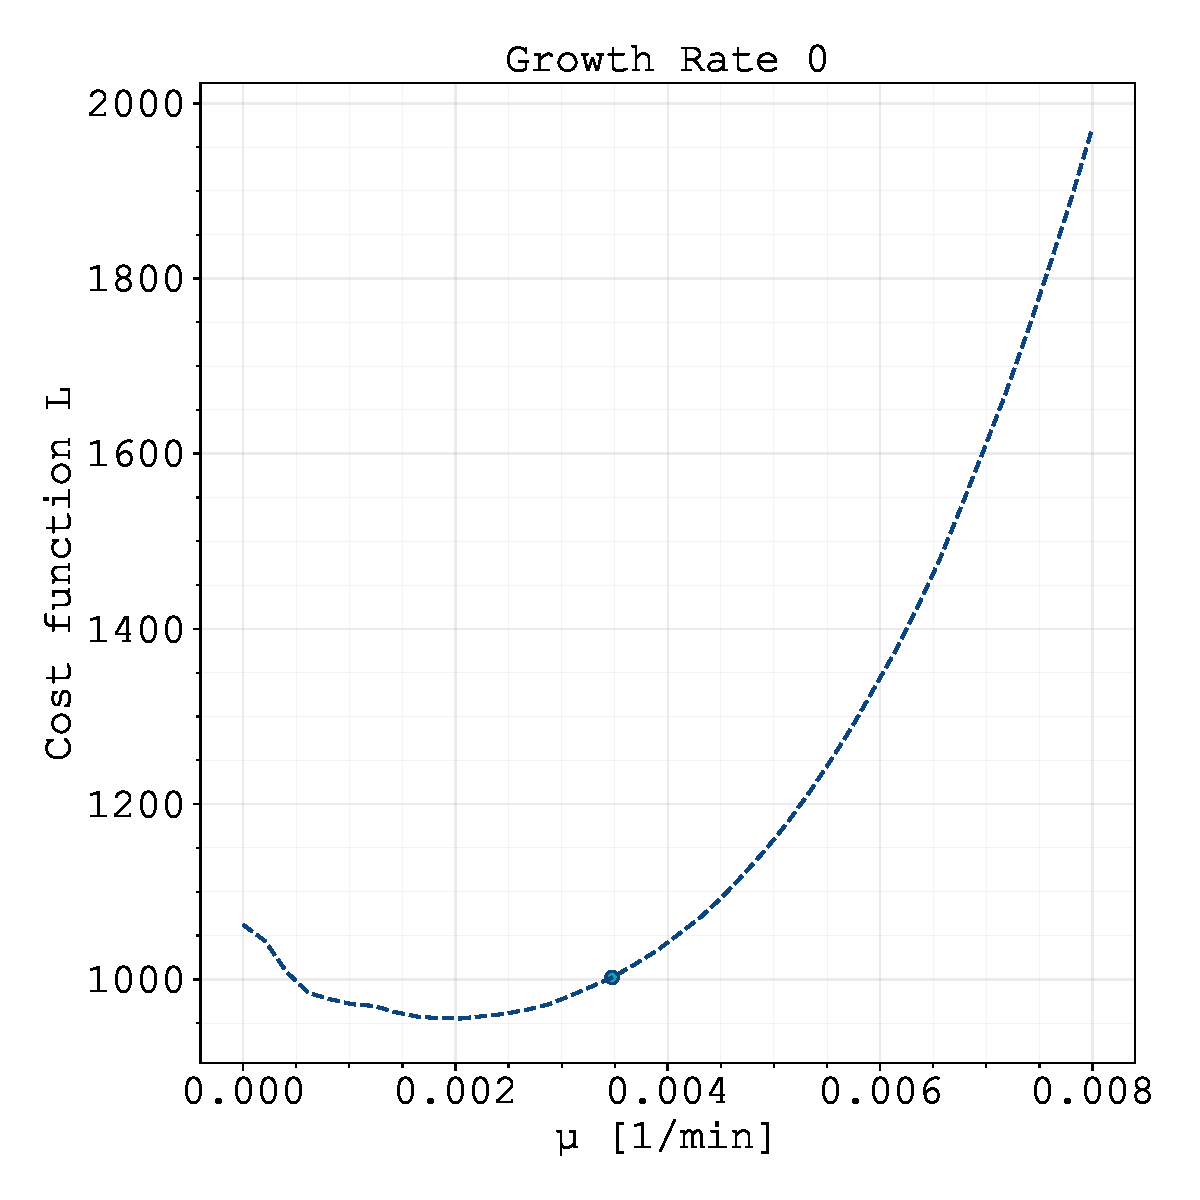
\includegraphics[width=0.33\textwidth]
        {figures/crm_fit/profiles/growth-rate-0.pdf}%
    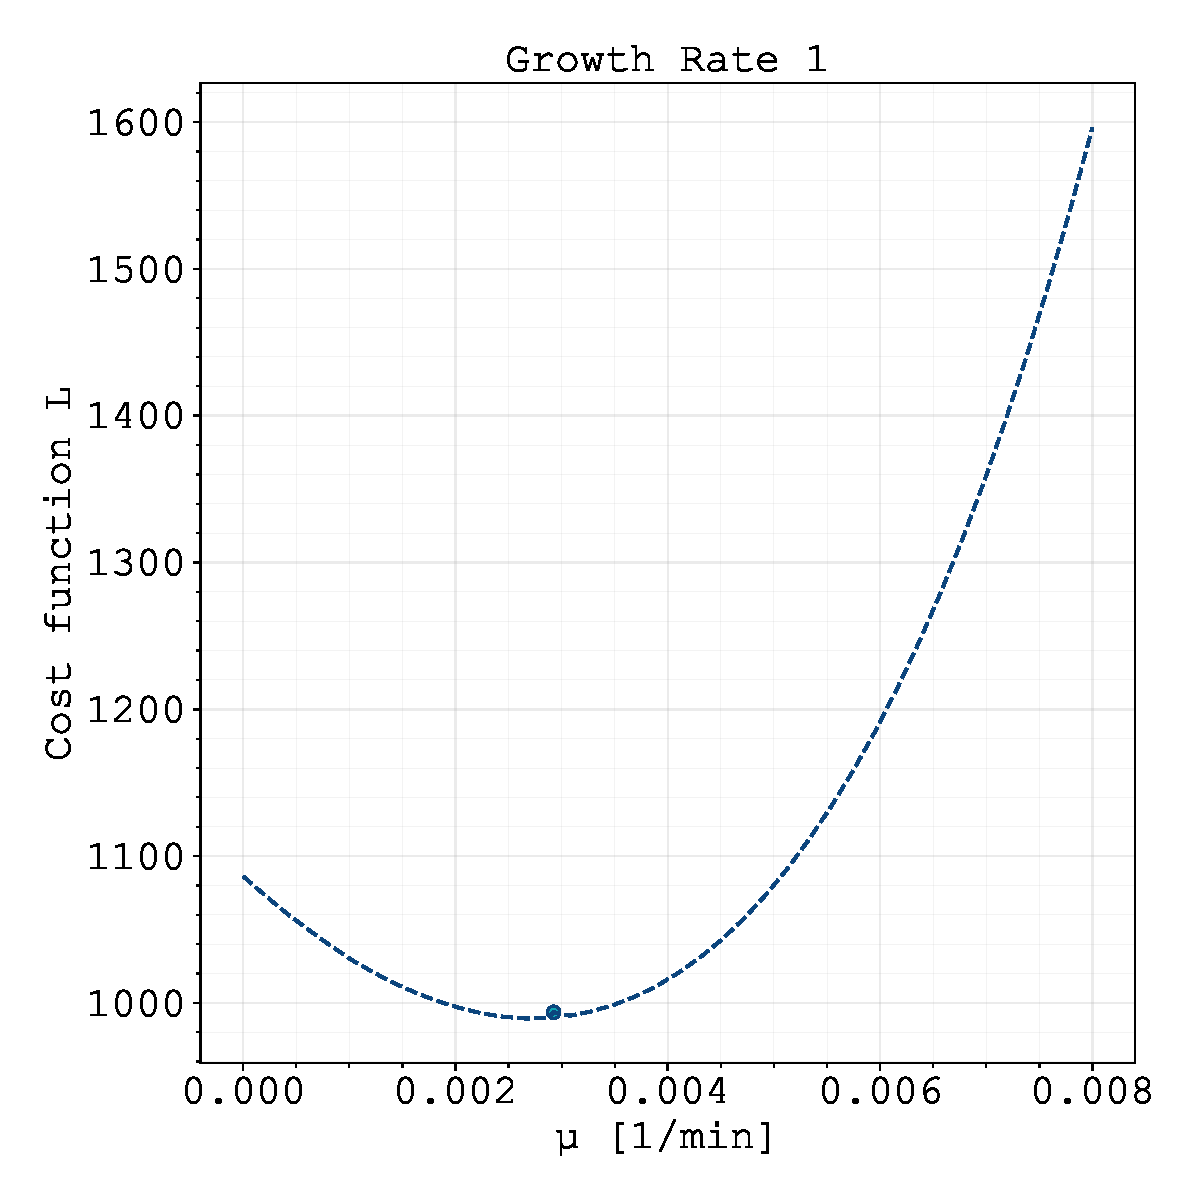
\includegraphics[width=0.33\textwidth]
        {figures/crm_fit/profiles/growth-rate-1.pdf}%
    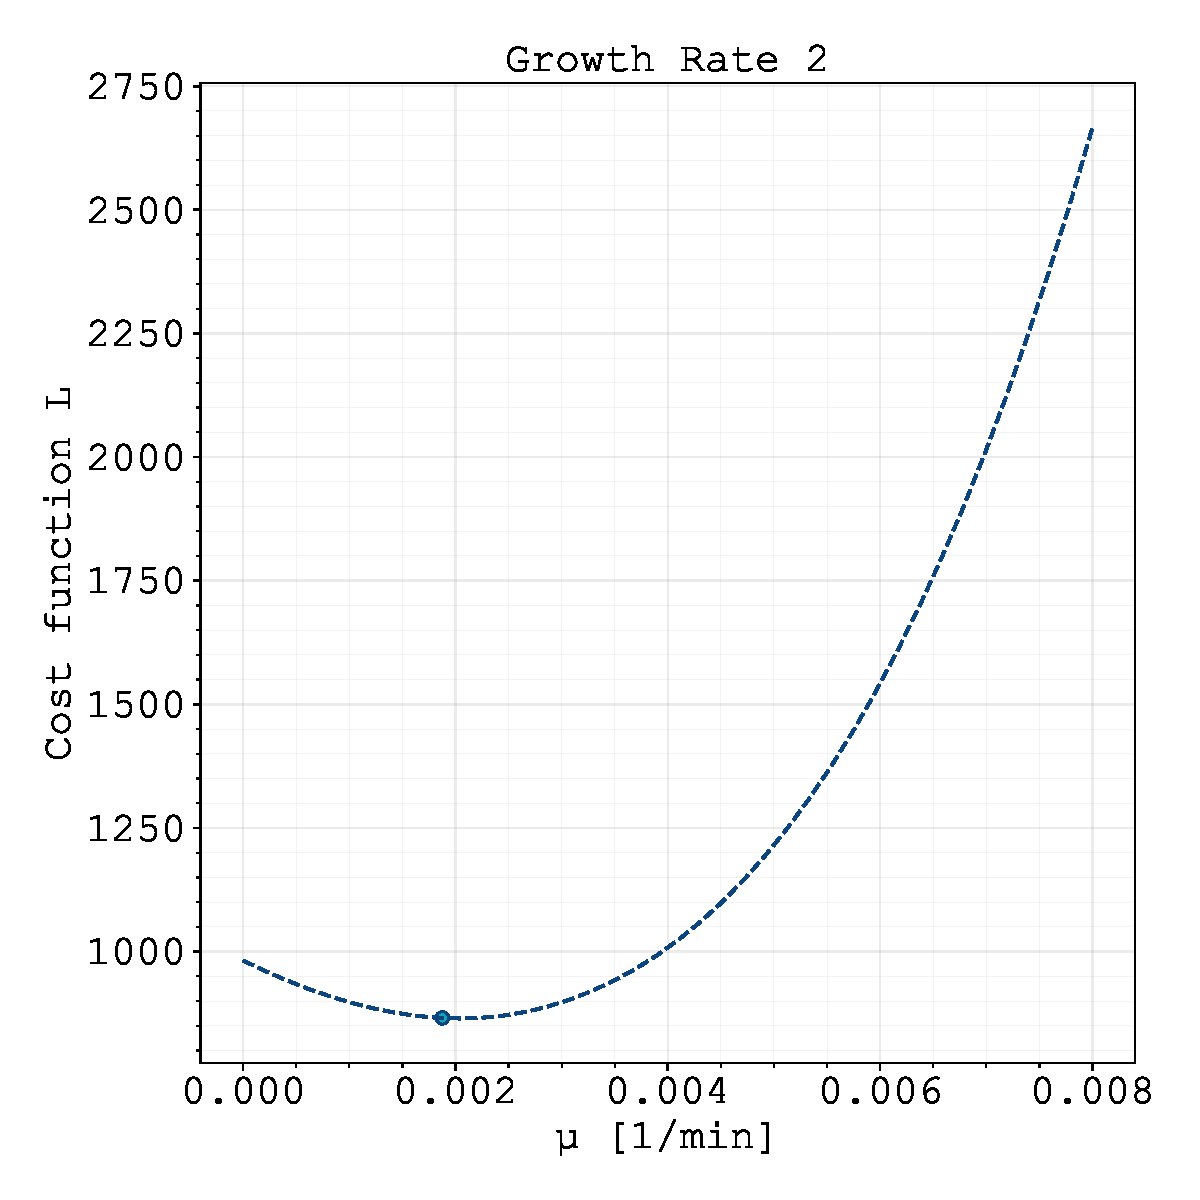
\includegraphics[width=0.33\textwidth]
        {figures/crm_fit/profiles/growth-rate-2.pdf}\\%
    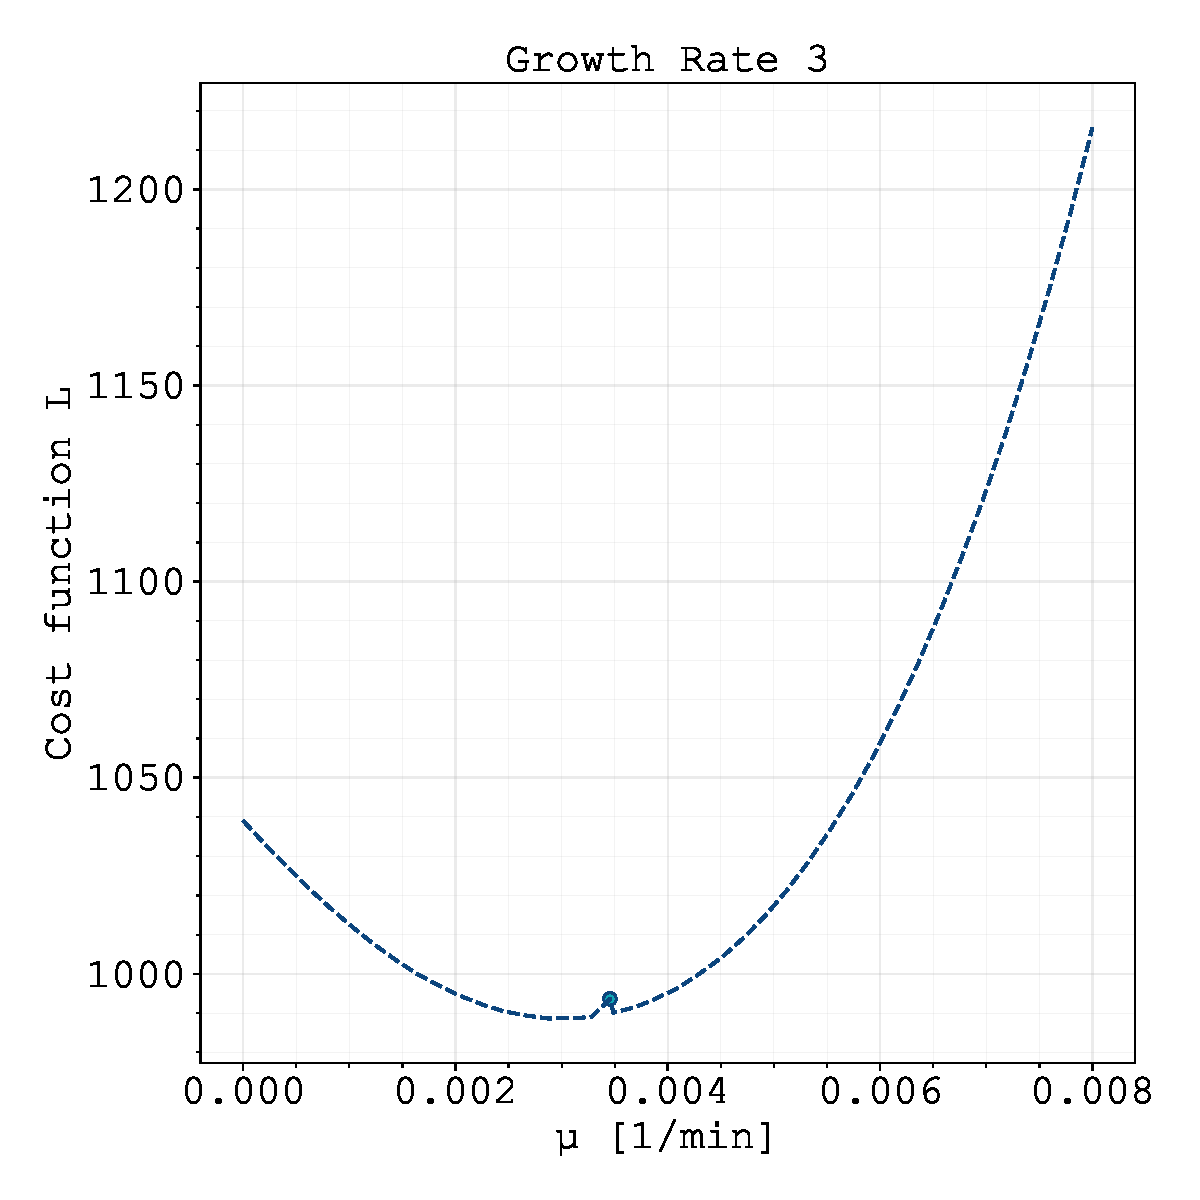
\includegraphics[width=0.33\textwidth]
        {figures/crm_fit/profiles/growth-rate-3.pdf}%
    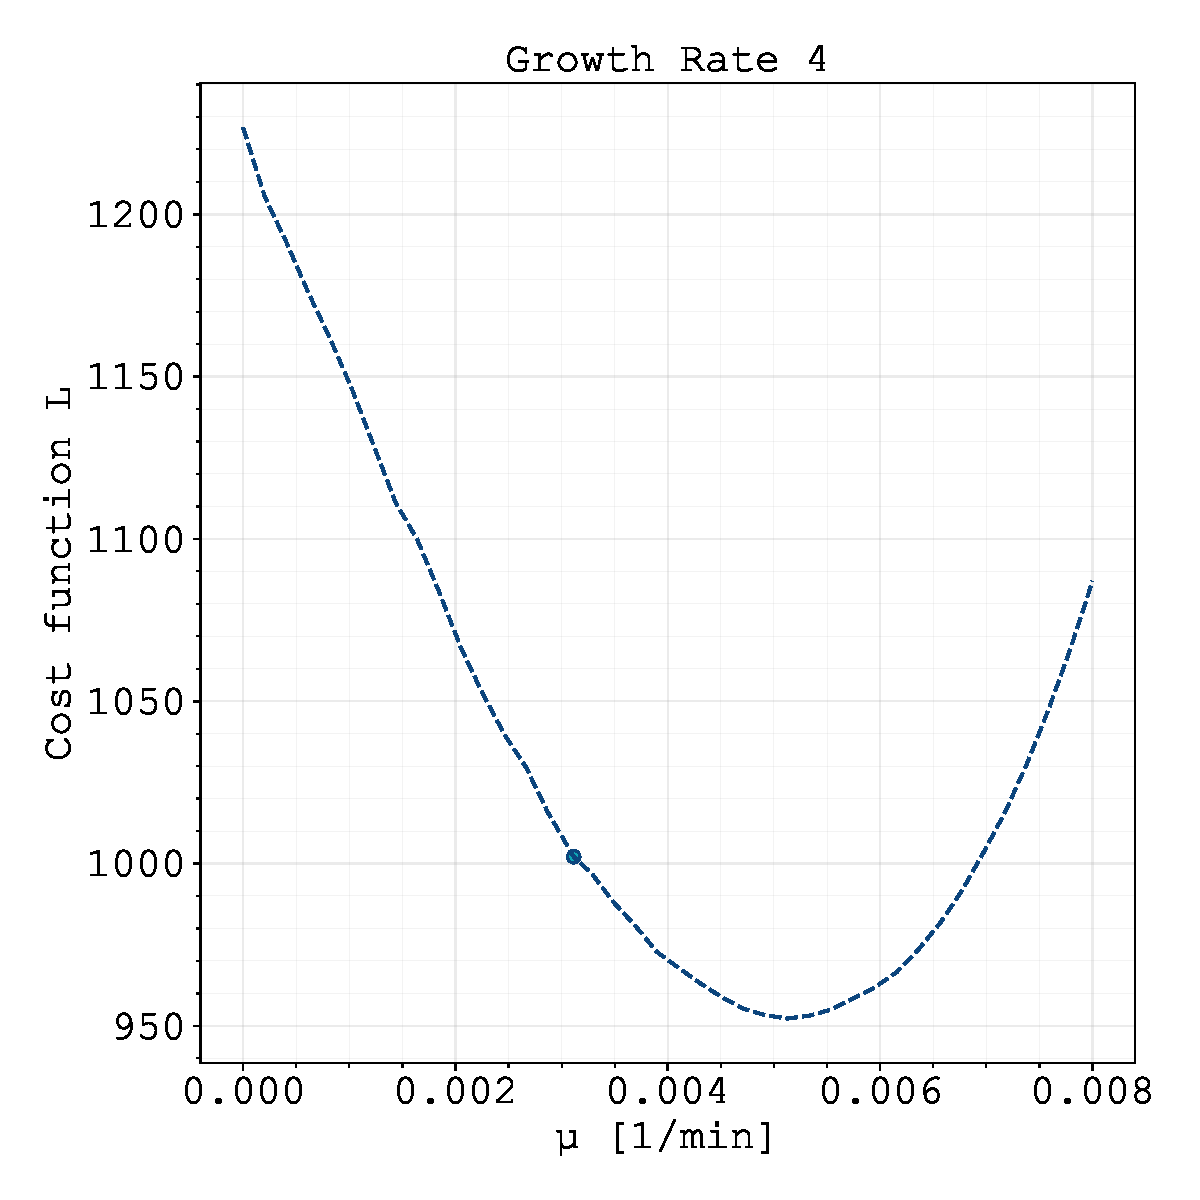
\includegraphics[width=0.33\textwidth]
        {figures/crm_fit/profiles/growth-rate-4.pdf}%
    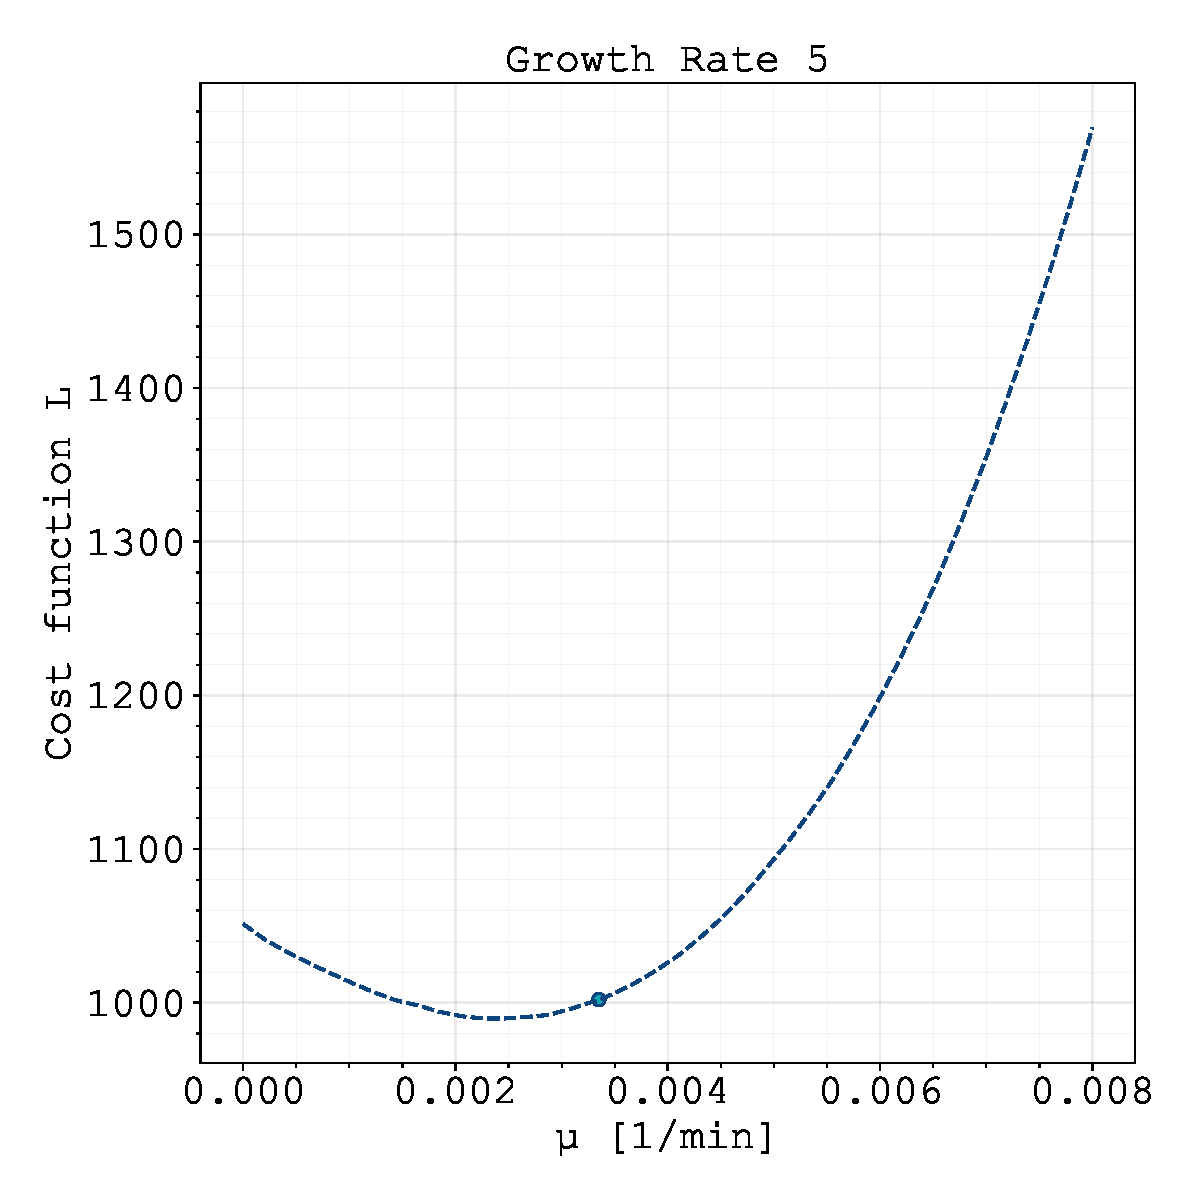
\includegraphics[width=0.33\textwidth]
        {figures/crm_fit/profiles/growth-rate-5.pdf}
    \caption{Parameter estimation of growth rates for individual cells}%TODO extend caption}
    \label{fig:parameter-estimates-supplement-growth-rates}
\end{figure}

\begin{table}
    \centering
    \begin{tabularx}{\textwidth}{l c c c c c c}
        \toprule
        % \multicolumn{6}{Growth Rates}\\
        Method & Cell $0$ & Cell $1$ & Cell $2$ & Cell $3$ & Cell $4$ & Cell $5$\\
        \midrule
        \ac{abm} & 0.0011527990 & 0.0014106040 & 0.0018761827 & 0.0016834959 & 0.0036106023 & 0.0015209642\\
        Direct   & 0.0014057073 & 0.0010807540 & 0.0023177727 & 0.0015120675 & 0.0020488179 & 0.0016726263\\
        % 0.0014057073 & 0.0010807540 & 0.0023177727 & 0.0015120675 & 0.0020488179 & 0.0016726263\\
        % direct & 0.0009785162 & 0.0012641432 & 0.0021701728 & 0.0015695889 & 0.0036255661 & 0.0018419186\\
        \bottomrule
    \end{tabularx}
    \caption{TODO}
\end{table}

%###################################################################################################
\subsection{Alternative Interaction Potential - Morse Potential}
The morse potential~\cite{Morse1929} is a common example of numerically inexpensive interaction
potential.
It was originally designed to describe the interaction of diatomic molecules but has since found use
in other areas~\cite{Breitwieser2021}.
It contains a repulsive and attractive part and is bound from above which makes it particularly
suitable for numerical simulations since unbound potentials can lead to large numerical deviations
thus compromising the prediction of the model.
The potential is of the form
\begin{equation}
    V(r) = V_0\left(1-e^{-\lambda(r-(R_1+R_2))}\right)^2
\end{equation}
and has 3 parameters.
The overall potential strength $V_0$, the radii of the particles $R_1,R_2$ and the potential
stiffness $\lambda$ which controls the rate of change as one travels along the radial axis.
We employ a spatial cutoff which sets the interaction strength to $0$ when exceeding a distance
$r\geq\xi$.


%###################################################################################################
\subsection{More Simulation Aspects (TODO)}
\label{section:supplement-more-simulation-aspects}
%TODO insert this into the discussion later
\begin{table}[H]
    \centering
    \def\arraystretch{1.3}
    \begin{tabularx}{\textwidth}{c l X}
        &\textbf{Aspect} & \textbf{Description}\\
        \toprule
        &\textbf{(C) Cellular}\\
        \midrule
        (1) & Rod-Shaped Mechanics &
            Rod-shaped bacteria are flexible rods which are able to freely move around (off-lattice
            approach) \cite{Takeuchi2005,Ursell2014,Amir2014_2}.\\
        (2) & Growth &
            Cells grow exponentially by inserting new material either along the circular part of the
            rod or at the tip~\cite{Robert2014,Takeuchi2005}.\\
        (3) & Differentiation &
            \textit{B.subtilis} is known to differentiate into matrix-producing and
            surfactin-producing cells \cite{vanGestel2015,Lpez2010}.\\
        (4) & Division &
            The formation and continuation of van Gogh bundles is driven by cell division
            \cite{vanGestel2015}.
            Bacteria can form multilayers during their growth phase \cite{Duvernoy2018}.\\
        (5) & Variable Parameters &
            Parameters for individual cells are not fixed values but rather taken from a
            distribution \cite{Koutsoumanis2013}.\\
        &\textbf{(CC) Cell-Cell Interactions}\\
        \midrule
        (6) & Adhesion &
            Bacteria adhere to each other at longer distances and attach when in close contact
            \cite{Verwey1947,Trejo2013}.
            The interaction between rods can be polarized \cite{Duvernoy2018}.\\
        (7) & Friction &
            Friction between cells \cite{Grant2014} can be asymmetrical \cite{Doumic2020}.\\
        &\textbf{(DC) Domain-Cell Interactions}\\
        \midrule
        (8) & External Forces &
            Bacteria tend to stick to surfaces \cite{vanLoosdrecht1989}.
            The extracellular gel exerts a force onto the cells \cite{Grant2014}.\\
        (9) & Extracellular Reactions &
            Bacteria can take up nutrients or possible secrete/take up signalling molecules
            \cite{Li2025}.\\
        \bottomrule
    \end{tabularx}
    \label{table:simulation-aspects-supplement}
    \caption{
        This table extends table~\ref{table:simulation-aspects} with additional observations.
        It has to be noted that this table includes more specific behaviour that might not be
        generalizable across all types of rod-shaped bacteria.
    }
\end{table}

\begin{itemize}
    \item new class of aspects: (DC) Domain-Cell Interactions
    \item List which aspects are here additionally
    \item discuss which of them might need specific models and can not be paired with others
    \item which can be bundled together without problems?
\end{itemize}

%###################################################################################################
\subsection{Performance (TODO)}
\label{section:supplement-performance}

\begin{itemize}
    \item Quadratic Scaling comes from more dense simulation
    \item Overall number of agents which can be simulated is satisfactory for current purposes
    \item Improvement from $1 \Rightarrow 2$ and $2\Rightarrow4$ threads; first is major; second
        only minor
    \item Flamegraph still shows much cycles running against hurdles::Barrier::wait $\Rightarrow$
        this leaves room for improvement
    \item Flamegraph also shows that $\approx 75\%$ of all cycles is related to actual work (not
        just waiting).
        In particular to update\_mechanics functions.
\end{itemize}

\begin{figure}
    \centering
    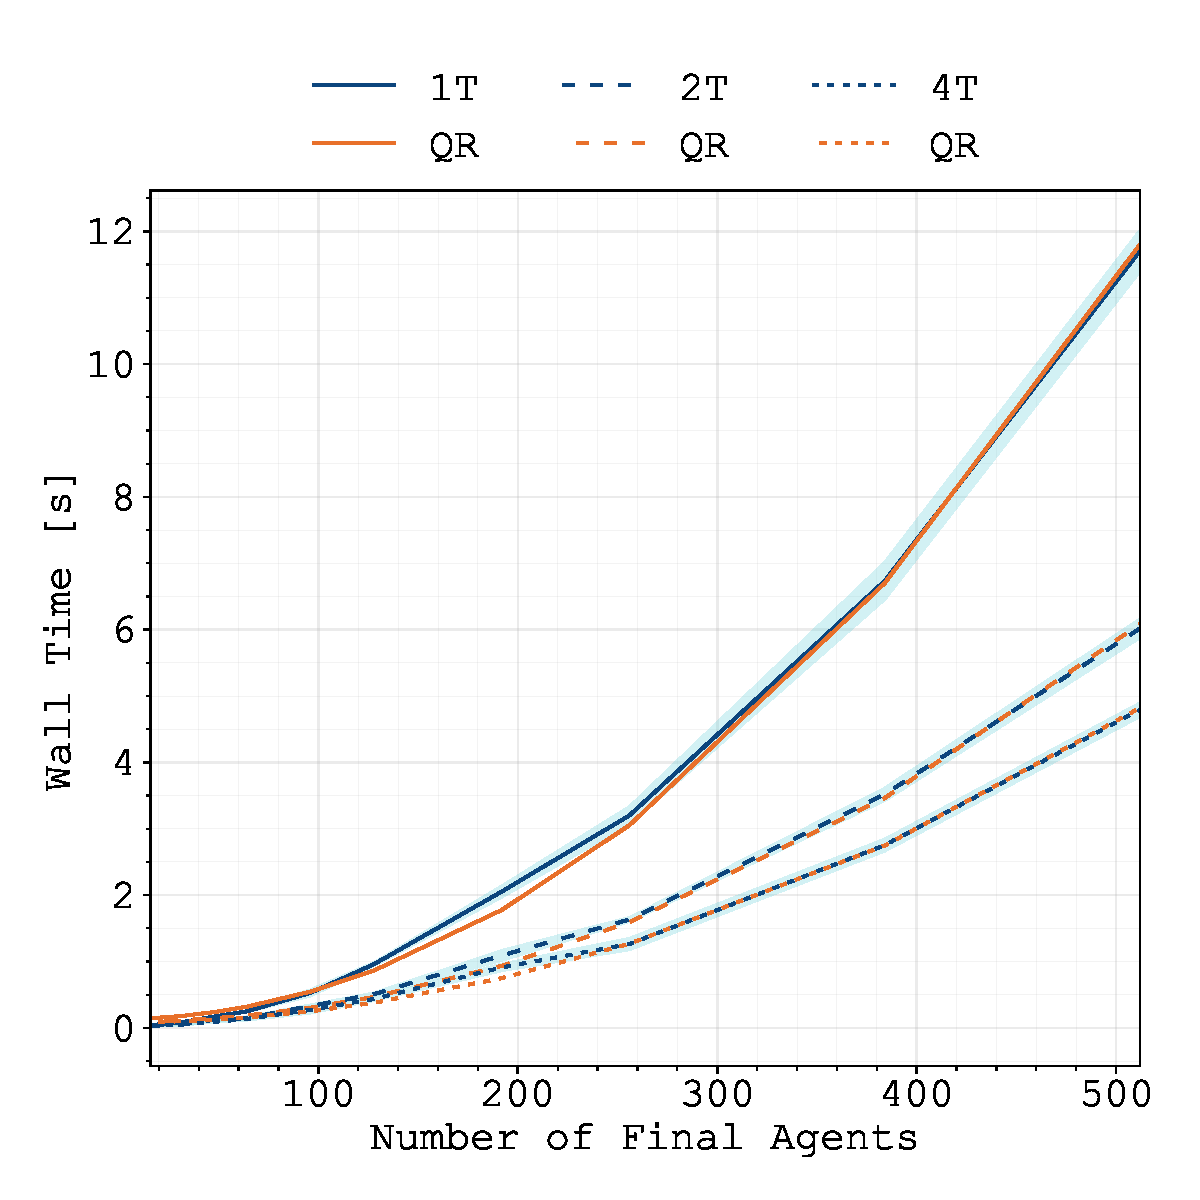
\includegraphics[width=0.49\textwidth]
        {docs/source/_static/performance/computation-time-with-initial-agents.pdf}
    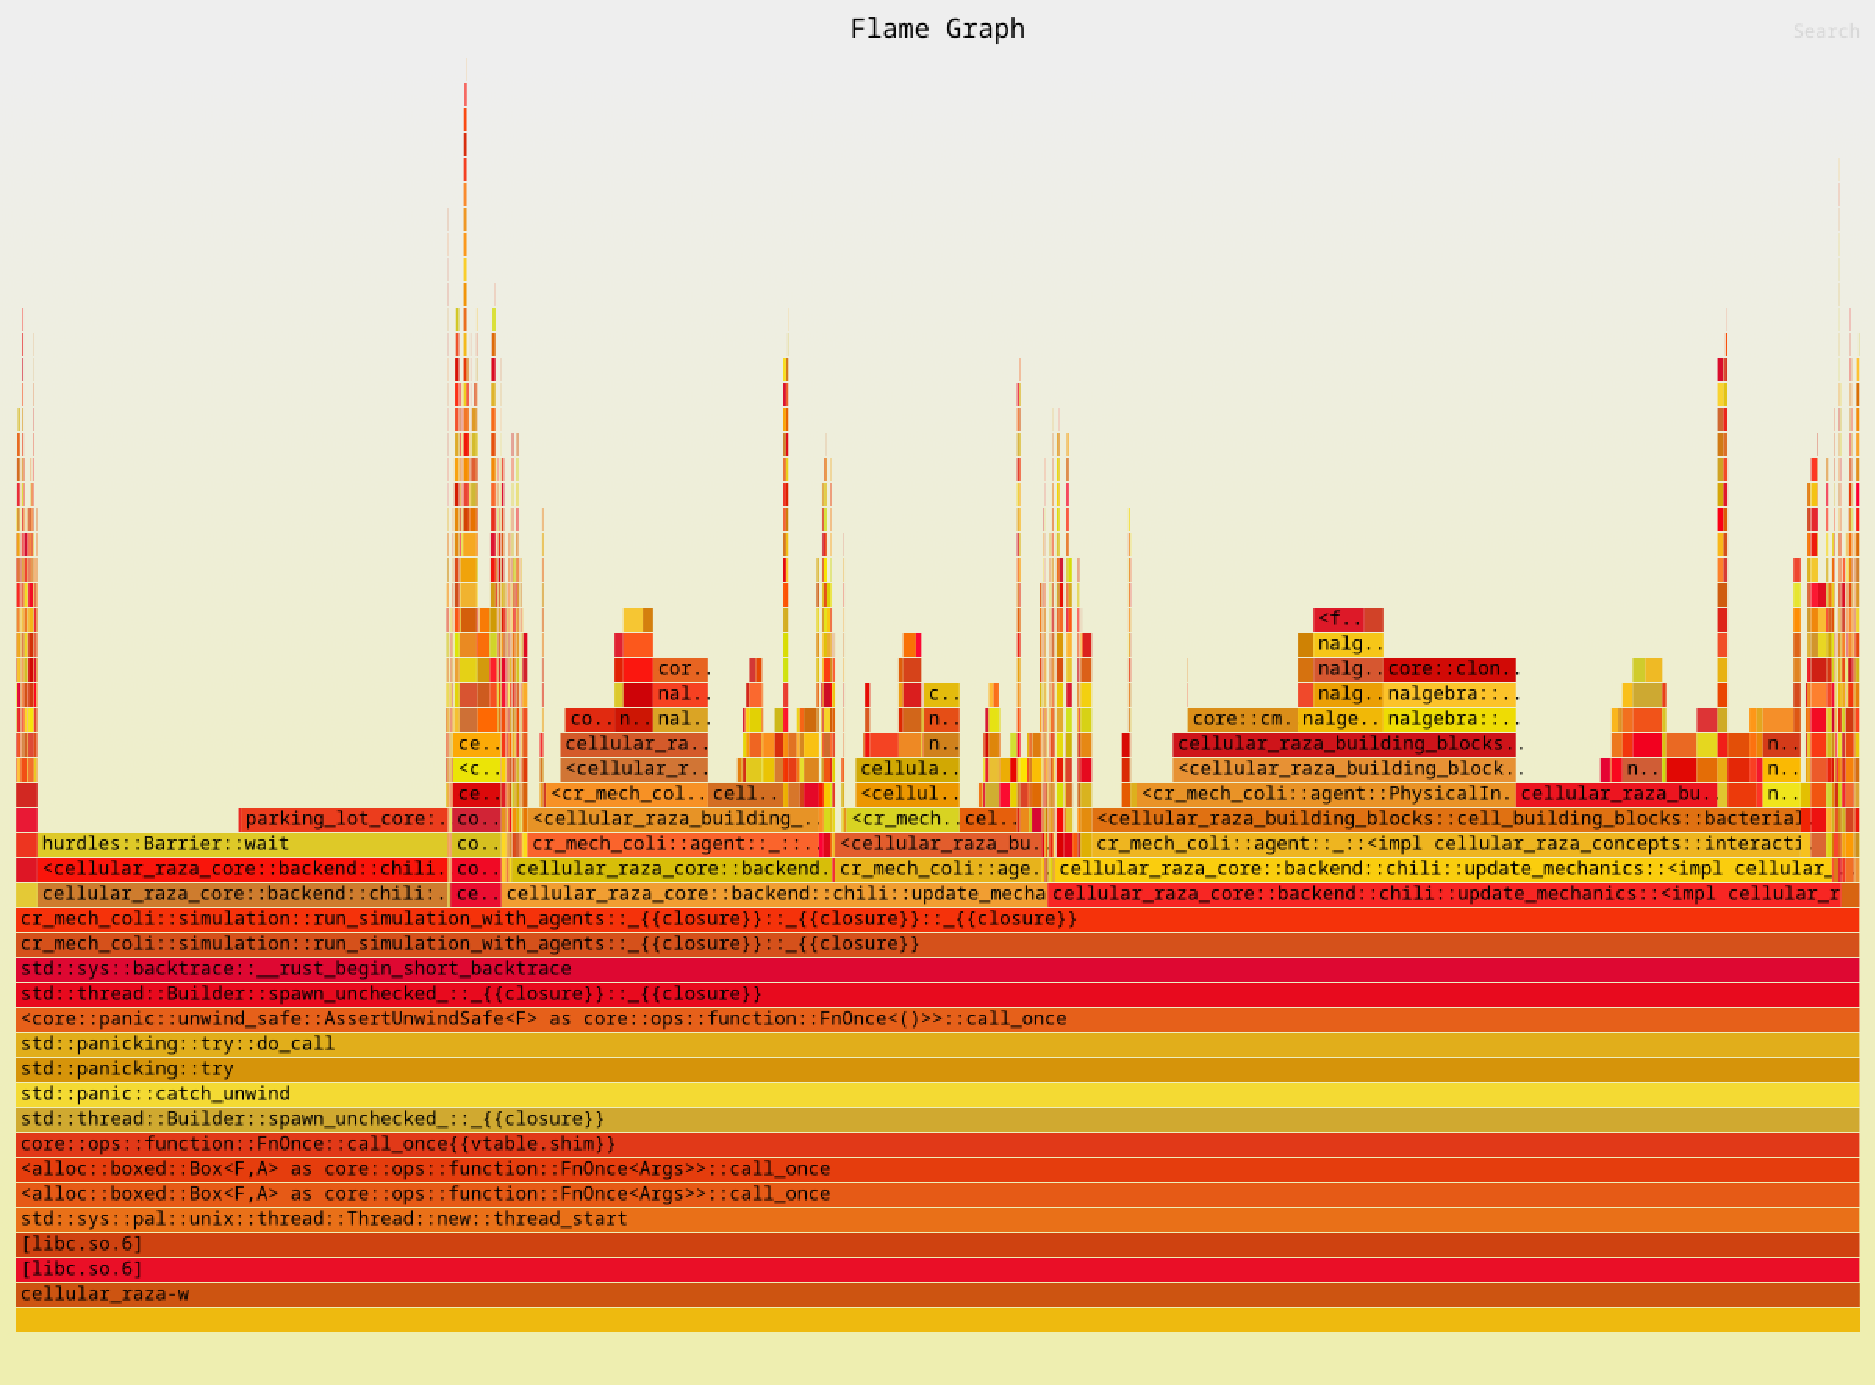
\includegraphics[width=0.49\textwidth]{docs/source/_static/performance/flamegraph.pdf}
    \caption{TODO}
    \label{fig:performance}
\end{figure}

\begin{figure}
    \centering
    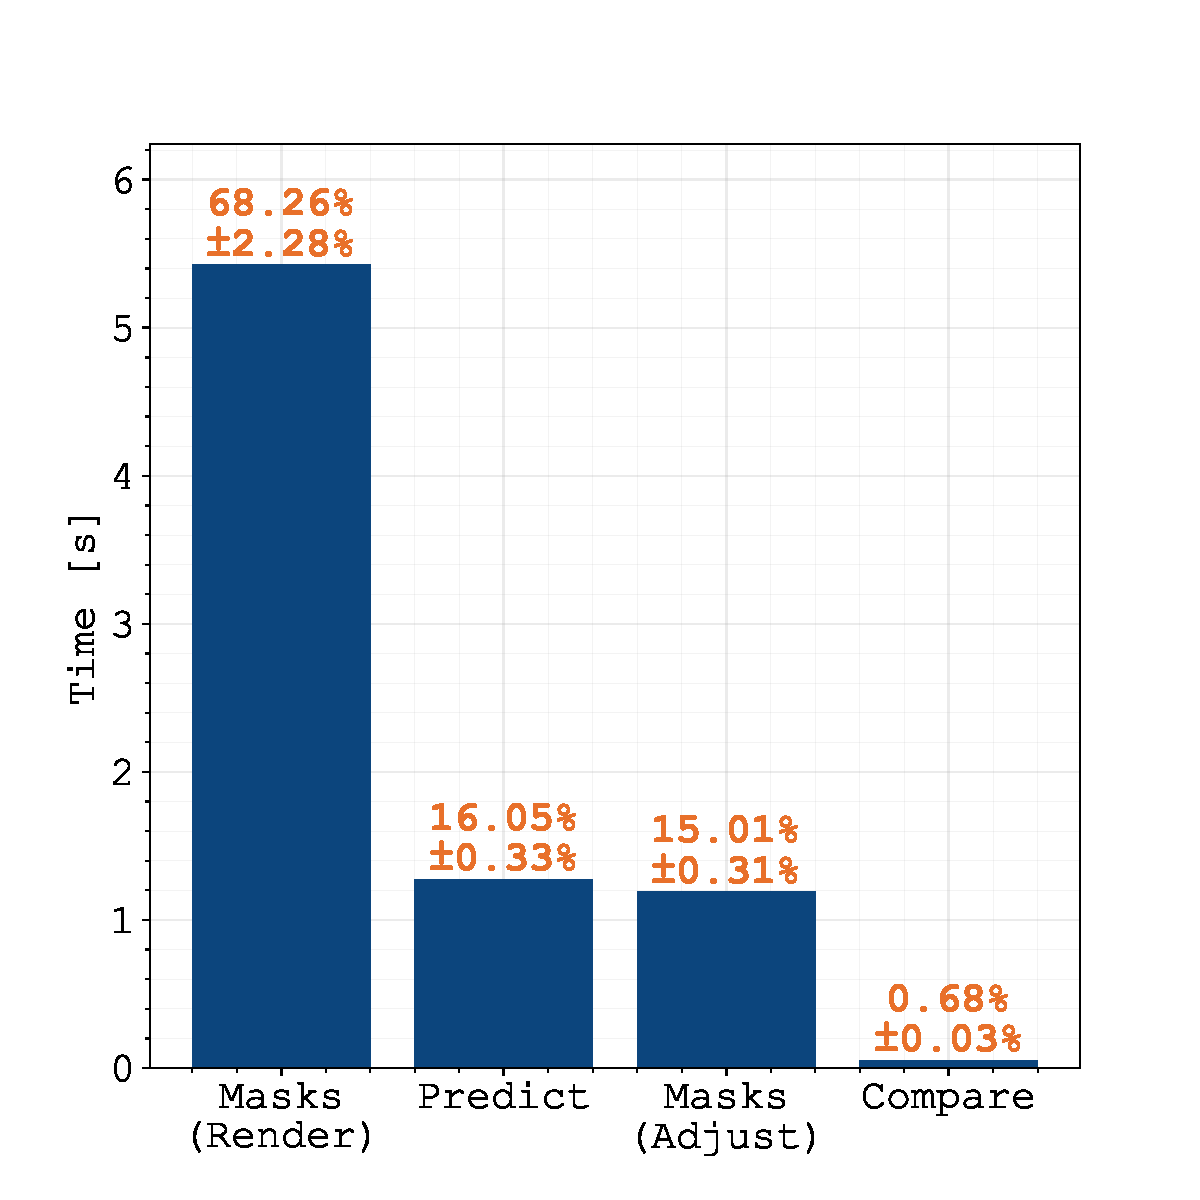
\includegraphics[width=0.5\textwidth]{figures/crm_divide/timings.pdf}%
    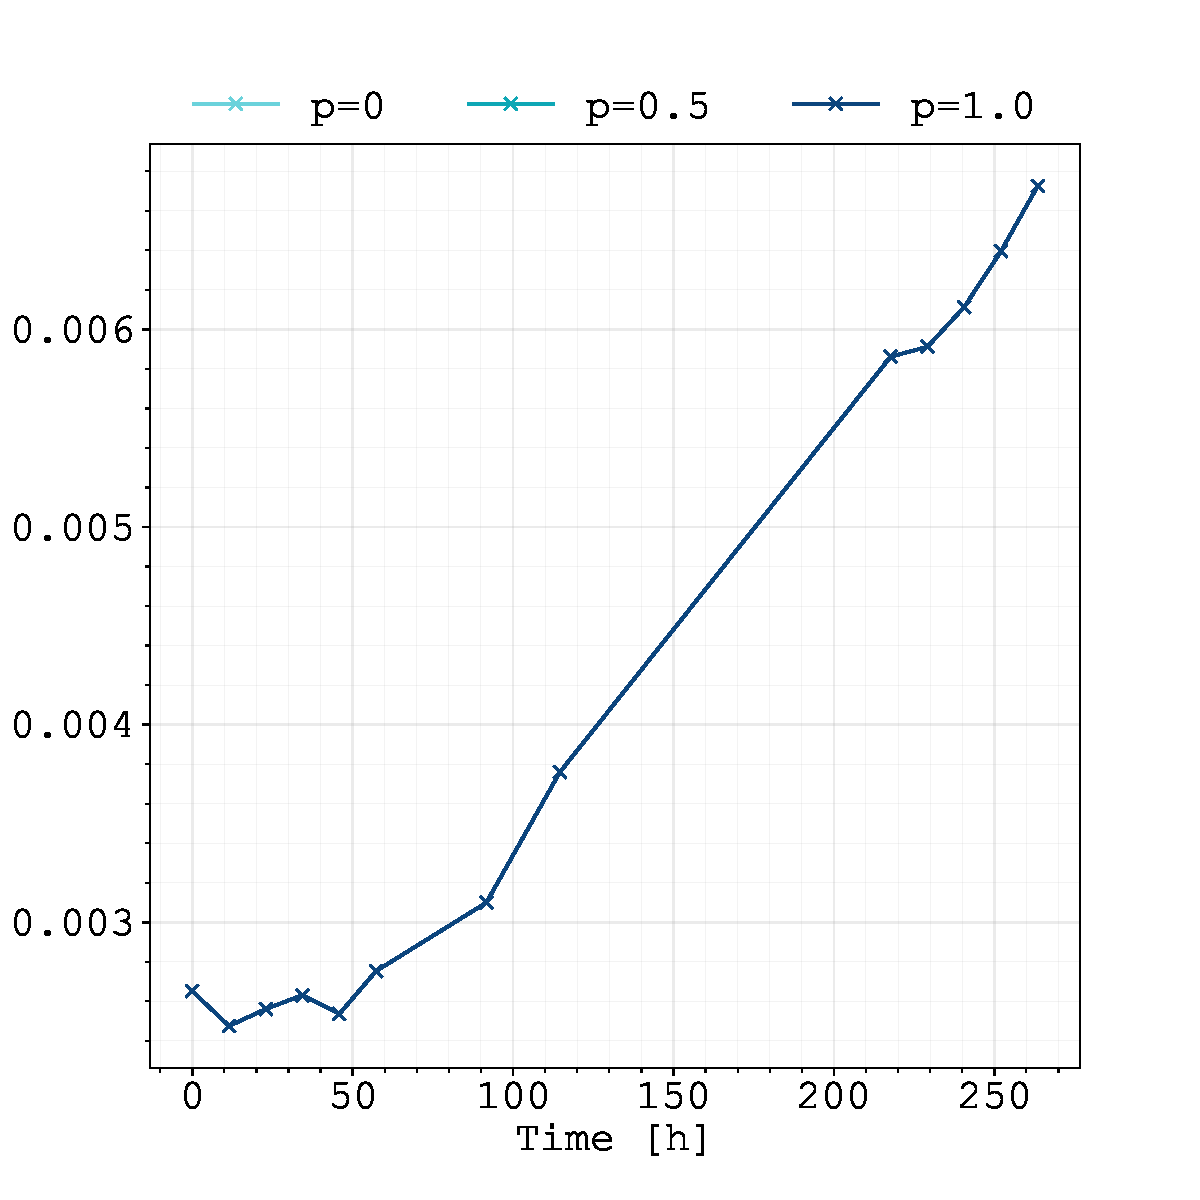
\includegraphics[width=0.5\textwidth]{figures/crm_divide/time-evolution.pdf}%
    \caption{TODO}
    \label{fig:timings-crm_divide}
\end{figure}

\end{document}
